\documentclass[a4paper,10pt,twoside]{book}

%%% preambulo
\input ../preambulo.tex
\input ../preambulo_counters.tex
\input ../preambulo_python.tex


\begin{document}

\frontmatter

% título
\title{Algoritmos e Programação I}
\author{Pedro H A Konzen}
\date{}
\maketitle

% ficha catolográfica
\ifisbook
~
\vspace{4.5in}
\hrule
Konzen, Pedro Henrique de Almeida \\
\indent\hspace{2em}Algoritmos e programação I: notas de aula / Pedro Henrique de Almeida Konzen. --{\the\year}. Porto Alegre.- {\the\year}. \\
\indent\hspace{2em}"Esta obra é uma edição independente feita pelo próprio autor." \\
\indent\hspace{2em}1. Algoritmos computacionais. 2. Programação de computadores. 3. Linguagem Python. \\
\hrule
\vspace{1cm}
\begin{center}
  \textit{Licença}\\CC-BY-SA 4.0.
\end{center}
\fi

% licença
\chapter*{Licença}\label{licenca}
\addcontentsline{toc}{chapter}{Licença}

Este texto é disponibilizado sob a Licença Atribuição-CompartilhaIgual 4.0 Internacional Creative Commons. Para visualizar uma cópia desta licença, visite 
\begin{center}
  \url{http://creativecommons.org/licenses/by-sa/4.0/deed.pt\_BR} 
\end{center}
ou mande uma carta para Creative Commons, PO Box 1866, Mountain View, CA 94042, USA.


% prefácio


\chapter*{Prefácio}\label{prefacio}
\addcontentsline{toc}{chapter}{Prefácio}

O site \href{https://www.notaspedrok.com.br}{notaspedrok.com.br} é uma plataforma que construí para o compartilhamento de minhas notas de aula. Essas anotações feitas como preparação de aulas é uma prática comum de professoras/es. Muitas vezes feitas a rabiscos em rascunhos com validade tão curta quanto o momento em que são concebidas, outras vezes, com capricho de um diário guardado a sete chaves. Notas de aula também são feitas por estudantes - são anotações, fotos, prints, entre outras formas de registros de partes dessas mesmas aulas. Essa dispersão de material didático sempre me intrigou e foi o que me motivou a iniciar o site.

Com início em 2018, o site contava com apenas três notas incipientes. De lá para cá, conforme fui expandido e revisando os materais, o site foi ganhando acessos de vários locais do mundo, em especial, de países de língua portugusa. No momento, conta com 13 notas de aula, além de minicursos e uma coleção de vídeos e áudios.

As notas de \emph{Algoritmos e Programação I} fazem uma introdução a algoritmos e programação de computadores com a linguagem {\python}. É pensada para estudantes de cursos de matemática e áreas afins.

Aproveito para agradecer a todas/os que de modo assíduo ou esporádico contribuem com correções, sugestões e críticas. ;-)

\begin{flushright}
  Pedro H A Konzen\\\url{https://www.notaspedrok.com.br}
\end{flushright}



% toc
\ifishtml
\clearpage
\phantomsection
\addcontentsline{toc}{chapter}{Conteúdo}
\fi
\tableofcontents


\mainmatter



\chapter{Introdução}\label{cap_intro}

Vamos começar executando nossas primeiras \emph{linhas de código} na linguagem de programação {\python}. Em um \emph{terminal} {\python} digitamos

\begin{lstlisting}
>>> print('Olá, mundo!')
\end{lstlisting}

Observamos que \lstinline+>>>+ é o símbolo do \lstinline+prompt de entrada+ e digitamos nossa \emph{instrução} logo após ele. Para executarmos a instrução digitada, teclamos \lstinline+<ENTER>+. Uma vez executada, o terminal apresentará as seguintes informações

\begin{lstlisting}
>>> print('Olá, mundo!')
Olá, mundo!
>>> 
\end{lstlisting}

Pronto! O fato do símbolo de \lstinline+prompt de entrada+ ter aparecido novamente, indica que a instrução foi completamente executada e o terminal está pronto para executar uma nova instrução.

A \emph{linha de comando} executada acima pede ao computador para imprimir no \lstinline+prompt de saída+ a frase \lstinline+Olá, mundo!+. O \emph{método} {\PYTHONprint} contém instruções para imprimir \emph{objetos} em um dispositivo de saída, no caso, imprime a frase na tela do computador.

Bem! Talvez imprimir no \lstinline+prompt de saída+ uma frase que digitamos no \lstinline+prompt de entrada+ possa parecer um pouco redundante no momento. Vamos considerar um outro exemplo, computar a soma dos números ímpares entre $0$ e $100$. Podemos fazer isso como segue

\begin{lstlisting}
>>> sum([i for i in range(100) if i%2 != 0])
2500
\end{lstlisting}

Oh! No momento, não se preocupe se não tenha entendido a linha de comando de entrada, ao longo dessas notas de aula isso vai ficando natural. A linha de comando de entrada usa o método {\PYTHONsum} para computar a soma dos elementos da \emph{lista} de números ímpares desejada. A lista é construída de forma \emph{iterada} e \emph{indexada} pela \emph{variável} \lstinline+i+, para \lstinline+i+ no intervalo/faixa de $0$ a $99$, se o resto da divisão de \lstinline+i+ por $2$ não for igual a $0$. Ok! O resultado computado foi $2500$.

De fato, a soma dos números ímpares de $0$ a $100$
\begin{equation}
  (1, 3, 5, \dotsc, 99)
\end{equation}
é a soma dos 50 primeiros elementos da progressão aritmética $a_i = 1 + 2i$, $i=0, 1, \ldots$, i.e.
\begin{align}
  \sum_{i=0}^{49}a_i &= a_0 + a_1 + \cdots + a_{49}\\
                     &= 1 + 3 + \cdots + 99\\
                     &= \frac{50(1 + 99)}{2}\\
                     &= 2500
\end{align}
como já esperado! Em {\python}, esta última conta pode ser computada como segue

\begin{lstlisting}
>>> 50*(1+99)/2
2500.0
\end{lstlisting}

% Este trabalho está licenciado sob a Licença Atribuição-CompartilhaIgual 4.0 Internacional Creative Commons. Para visualizar uma cópia desta licença, visite http://creativecommons.org/licenses/by-sa/4.0/deed.pt_BR ou mande uma carta para Creative Commons, PO Box 1866, Mountain View, CA 94042, USA.

\chapter{Linguagem de Programação}\label{cap_lingua}
\thispagestyle{fancy}

\section{Computador}\label{cap_lim_sec_computador}

\begin{flushright}
  [YouTube] | [Vídeo] | [Áudio] | [Contatar]
\end{flushright}

Um computador\footnote{Consulte \href{https://pt.wikipedia.org/wiki/Computador}{Wikipédia: Computador} para uma introdução sobre a história e outras questões sobre computadores.} é um \emph{sistema computacional} de elementos físicos (\emph{hardware}) e elementos lógicos (\emph{software}).

O \emph{hardware} são suas partes mecânicas, elétricas e eletrônicas como: fonte de energia, teclado, mouse/painel tátil, monitor/tela, dispositivos de armazenagem de dados (HDD, {\it hard disk drive}; SSD, {\it solid-state drive}; RAM, {\it random-access memory}; etc.), dispositivos de processamento (CPU, {\it central processing unit}, GPU, {\it graphics processing unit}), conectores de dispositivos externos (microfone, caixa de som, fone de ouvido, USB, etc.), placa mãe, etc..

O \emph{software} é toda a informação processada pelo computador, qualquer código executado e qualquer dado usado nas computações.

\begin{figure}[H]
  \centering
  \includegraphics[width=\textwidth]{./cap_lingua/dados/fig_arqVonNeumann/main}
  \caption[Arquitetura de von Neumann]{Arquitetura de computador de von Neumann.}
  \label{cap_lim_sec_computador:fig:arqVonNeumann}
\end{figure}

Os computadores que comumente utilizamos seguem a arquitetura de John von Neumann\footnote{John von Neumann, 1903 - 1957, matemático húngaro, naturalizado estadunidense. Fonte: \href{https://pt.wikipedia.org/wiki/John_von_Neumann}{Wikipédia}.}, que consiste em dispositivo(s) de entrada de dados, unidade(s) de processamento, unidade(s) de memória e dispositivo(s) de saída de dados (Figura~\ref{cap_lim_sec_computador:fig:arqVonNeumann}).

\begin{itemize}
\item \emph{Dispositivos de entrada e saída}

  São elementos do computador que permitem a comunicação humana (usuária(o)) com a máquina.

  \begin{itemize}
  \item \emph{Dispositivos de entrada}

    São elementos que permitem o fluxo de informação da(o) usuária(o) para a máquina. Exemplos são: teclado, mouse/painel tátil, microfone, etc.

  \item \emph{Dispositivos de saída}

    São elementos que permitem o fluxo de informação da máquina para a(o) usuária(o). Exemplos são: monitor/tela, alto-falantes, luzes espia, etc.
  \end{itemize}

\item \emph{Unidade central de processamento}

  A \emph{CPU} (do inglês, {\it Central Processing Unit}) é o elemento de processa as informações e é composta de \emph{unidade de controle}, \emph{unidade lógica e aritmética} e de \emph{memória cache}.

  \begin{itemize}
  \item \emph{Unidade de controle}

    Coordena as execuções do processador: busca e decodifica instruções, lê e escreve no {\it cache} e controla o fluxo de dados.

  \item \emph{Unidade lógica/aritmética}

    Executa as instruções operações lógicas e aritméticas, por exemplo: executar a adição, multiplicação, testar se dois objetos são iguais, etc.

  \item \emph{Memória cache}

    Memória interna da CPU muito mais rápida que as memórias RAM e dispositivos e armazenamento HDD/SSD. É um dispositivo de memória de pequena capacidade e é utilizada como memória de curto prazo e diretamente acessada.
  \end{itemize}

\item \emph{Unidades de memória}

  As unidades de memória são elementos que permitem o armazenamento de dados/objetos. Como memória principal tem-se a \emph{ROM} (do inglês, {\it Read Only Memory}) e a \emph{RAM} (do inglês, {\it Random Access Memory}) e como memória de massa/secundária tem-se HDD, SSD, entre outras.

\item \emph{Memória ROM}

  A memória ROM é utilizada para armazenamento de dados/objetos necessários para dar início ao funcionamento do computador. Por exemplo, é onde a BIOS (dos inglês, {\it Basic Input/Output System}, Sistema Básico de Entrada e Saída) é armazenada. Ao ligarmos o computador este programa é iniciado e é responsável por fazer o gerenciamento inicial dos diversos dispositivos do computador e carregar o \emph{sistema operacional} (conjunto de programas cuja função é de gerenciar os recursos do computador e controlar a execução de programas).

\item \emph{Memória RAM}

  Memória de acesso rápido utilizada para dados/objetos de uso frequente durante a execução de programas. É uma memória volátil, i.e. toda a informação guardada nela é perdida quando o computador é desligado.

\item \emph{Memória de massa/secundária}

  Memória de massa ou secundária são usadas para armazenar dados/objetos por período longo. Normalmente, são dispositivos HDD ou SSD, os dados/objetos são guardados mesmo que o computador seja desligado e contém grande capacidade de armazenagem.   
\end{itemize}

Os \emph{software} são os elementos lógicos de um sistema computacional, são programas de computadores que contém as instruções que gerenciam o \emph{hardware} para a execução de tarefas específicas, por exemplo, imprimir um texto, gravar áudio/vídeo, resolver um problema matemático, etc. Programar é o ato de criar programas de computadores.

\subsection{Linguagem de programação}

As informações fluem no computador codificadas como registros de {\it bits}\footnote{Usualmente de tamanho $64$-{\it bits}.} (sequência de zeros ou uns). Há registros de instrução e de dados. Programar diretamente por registros é uma tarefa muito difícil, o que levou ao surgimento de linguagens de programação. Uma \emph{linguagem de programação}\footnote{Código de programação, código de máquina ou linguagem de máquina.} é um método padronizado para escrever instruções para execução de tarefas no computador. As instruções escritas em uma linguagem são interpretadas e/ou compiladas por um software (interpretador ou compilador) da linguagem que decodifica as instruções em registros de instruções e dados, os quais são efetivamente executados na máquina.

Existem várias linguagens de programação disponíveis e elas são classificadas por diferentes características. Uma \emph{linguagem de baixo nível} (por exemplo, \href{https://pt.wikipedia.org/wiki/Linguagem_assembly}{Assembly}) é aquela que se restringe às instruções executadas diretamente pelo processador, enquanto que uma \emph{linguagem de alto nível} contém instruções mais complexas e abstratas. Estas contém sintaxe mais próxima da linguagem humana natural e permitem a manipulação de objetos mais abstratos. Exemplos de linguagens de alto nível são: \href{https://pt.wikipedia.org/wiki/BASIC}{Basic}, \href{https://pt.wikipedia.org/wiki/Java\_(linguagem\_de\_programa\%C3\%A7\%C3\%A3o)}{Java}, \href{https://pt.wikipedia.org/wiki/JavaScript}{Javascript}, \href{https://pt.wikipedia.org/wiki/MATLAB}{MATLAB}, \href{https://pt.wikipedia.org/wiki/PHP}{PHP}, \href{https://pt.wikipedia.org/wiki/R\_(linguagem_de_programa\%C3\%A7\%C3\%A3o)}{R}, \href{https://pt.wikipedia.org/wiki/C\%2B\%2B}{C/C++}, {\python}, etc.

Em geral, não existe uma melhor linguagem, cada uma tem suas características que podem ser mais ou menos adequadas conforme o programa que se deseja desenvolver. Por exemplo, para um site de internet, linguagens como \href{https://pt.wikipedia.org/wiki/JavaScript}{Javascript} e \href{https://pt.wikipedia.org/wiki/PHP}{PHP} são bastante úteis, mas não no desenvolvimento de modelagem matemática e computacional. Nestes casos, \href{https://pt.wikipedia.org/wiki/C\%2B\%2B}{C/C++} é uma linguagem mais apropriada por conter várias estruturas de programação que facilitam a modelagem computacional de problemas científicos. Agora, \href{https://pt.wikipedia.org/wiki/R\_(linguagem_de_programa\%C3\%A7\%C3\%A3o)}{R} é uma linguagem de alto nível com diversos recursos dedicados às áreas de ciências de dados e estatística. Usualmente, utiliza-se mais de uma linguagem no desenvolvimento de programas mais avançados. A ideia é de explorar o melhor de cada linguagem na criação de programas eficientes na resolução dos problemas de interesse.

Nestas notas de aula, {\python} é a linguagem escolhida para estudarmos algoritmos e programação. Trata-se de uma linguagem de alto nível, \emph{interpretada}, \emph{dinâmica} e \emph{mutiparadigma}. Foi lançada por Guido van Rossum\footnote{Guido van Rossum, 1956-, matemático e programador de computadores holandês. Fonte: \href{https://pt.wikipedia.org/wiki/Guido\_van\_Rossum}{Wikipédia}.} em 1991 e, atualmente, é desenvolvida de forma comunitária, aberta e gerenciada pela ONG \href{https://pt.wikipedia.org/wiki/Python_Software_Foundation}{Python Software Foundation}. A linguagem foi projetada para priorizar a legibilidade do código. Parte da filosofia da linguagem é descrita pelo poema \href{https://pt.wikipedia.org/wiki/Zen_de_Python}{The Zen of Python}. Pode-se lê-lo pelo {\it easter egg} {\python}:
\begin{lstlisting}
  >>> import this
\end{lstlisting}

\begin{itemize}
\item Linguagem interpretada

  {\python} é uma linguagem interpretada. Isso significa que o \emph{código-fonte} escrito em linguagem {\python} é interpretado por um programa (interpretador {\python}). Ao executar-se um código, o interpretador lê uma linha do código, decodifica-a como registros para o processador que os executa. Executada uma linha, o interpretador segue para a próxima até o código ter sido completadamente executado.

\item Linguagem compilada

  Em uma linguagem compilada, como \href{https://pt.wikipedia.org/wiki/C\%2B\%2B}{C/C++}, há um programa chamado de \emph{compilador} (em inglês, {\it compiler}) e outro de \emph{ligador} (em inglês, {\it linker}). O primeiro, cria um programa-objeto a partir do código e o segundo gerencia sua ligação com eventuais bibliotecas computacionais que ele possa depender. O programa-objeto (também chamado de executável) pode então ser executado pela máquina.
\end{itemize}

Em geral, a execução de um programa compilado é mais rápida que a de um código interpretado. De forma simples, isso se deve ao fato de que nesse a interpretação é feita toda de uma vez e não precisa ser refeita na execução de cada linha de código, como no segundo caso. Por outro lado, a compilação de códigos-fonte grandes pode ser bastante demorada fazendo mais sentido quando ele é compilado uma vez e o programa-objeto executado várias vezes. Além disso, linguagens interpretadas podem usar bibliotecas de programas pré-compiladas. Com isso, pode-se alcançar um bom balanceamento entre tempo de desenvolvimento e de execução do código.

O interpretador {\python} também pode ser usado para compilar o código para um arquivo \emph{bytecode}, este é executado muito mais rápido do que o código-fonte em si, pois as interpretações necessárias já foram feitas. Mais adiante, vamos estudar isso de forma mais detalhada.

\begin{itemize}
\item Linguagem de tipagem dinâmica

  {\python} é uma linguagem de tipagem dinâmica. Nela, os dados não precisam ser explicitamente tipificados no código-fonte e o interpretador os tipifica com base em regras da própria linguagem. Ao executar operações com os dados, o interpretador pode alterar seus tipos de forma dinâmica.

\item Linguagem de tipagem estática

  \href{https://pt.wikipedia.org/wiki/C\%2B\%2B}{C/C++} é um exemplo de uma linguagem de tipagem estática. Em tais linguagens, os dados devem ser explicitamente tipificados no código-fonte com base nos tipos disponíveis. A retipificação pode ocorrer, mas precisa estar explicitamente definida no código.
\end{itemize}

Existem vários \emph{paradigmas de programação} e a linguagem {\python} é multiparadigma, i.e. permite a utilização de mais de um no código-fonte. Exemplos de paradigmas de programação são: \emph{estruturada}, \emph{orientada a objetos}, \emph{orientada a eventos}, etc.. Na maior parte destas notas de aulas, vamos estudar algoritmos para linguagens de programação estruturada. Mais ao final, vamos introduzir aspectos de linguagens orientada a objetos. Estes são paradigmas de programação fundamentais e suas estruturas são importantes na programação com demais paradigmas disponíveis em programação de computadores.

\subsection{Instalação e execução}

{\python} é um \emph{software aberto}\footnote{Consulte a licença de uso em \url{https://docs.python.org/3/license.html}.} e está disponível para vários sistemas operacionais ({\linux}, macOS, Windows, etc.) no seu site oficial
\begin{center}
  \url{https://www.python.org/}
\end{center}
Também, está disponível (gratuitamente) na loja de aplicativos dos sistemas operacionais mais usados. Esta costuma ser a forma mais fácil de instalá-lo na sua máquina, consulte a loja de seus sistema operacional. Ainda, há plataformas e IDEs\footnote{IDE, do inglês, {\it Integrated Development enviroment}, ambiente de desenvolvimento integrado} {\python} disponíveis, consulte, como por exemplo, \href{https://www.anaconda.com/}{Anaconda}.

A execução de um código {\python} pode ser feita de várias formas.

\begin{itemize}
\item \emph{Execução iterativa via terminal}

  Em terminal {\python} pode-se executar instruções/comandos de forma iterativa. Por exemplo:
  \begin{lstlisting}
    >>> print('Olá, mundo!')
    Olá, mundo!
    >>> 
  \end{lstlisting}

  O símbolo \lstinline+>>>+ denota o \emph{prompt de entrada}, onde uma instrução {\python} pode ser digitada. Após digitar, o comando é executada teclando \lstinline+<ENTER>+. Caso o comando tenha alguma saída de informação, como no caso acima, esta aparecerá, por padrão, no \emph{prompt de saída}, logo abaixo a linha de comando executada. Um novo símbolo de prompt de entrada aparece ao términa da execução anterior.

\item \emph{Execução de um {\it script}}

  Para códigos com várias linhas de instruções é mais adequado utilizar um aquivo de {\it script} {\python}. Usando-se um editor de texto ou um IDE ditam-se as linhas de comando em um arquivo \lstinline+.py+. Então, {\it script} pode ser executado em um terminal de seu sistema operacional utilizando-se o interpretador {\python}. Por exemplo, assumindo que o código for salvo do arquivo \lstinline+path_to_arq/arq.py+, pode-se executá-lo em um terminal do sistema com
  \begin{lstlisting}
    $ python3 path_to_arq/arq.py 
  \end{lstlisting}%$
  

  IDEs para {\python} fornecem uma ambiente integrado, contendo um campo para escrita do código e terminal {\python} integrado. Consulte, por exemplo, o IDE {\spyder}:
  \begin{center}
    \url{https://www.spyder-ide.org/}
  \end{center}

\item \emph{Execução em um {\it notebook}}

  {\it Notebooks} {\python} são uma boa alternativa para a execução de códigos em um ambiente colaborativo/educativo. Por exemplo, {\jupyter} é um notebook que roda em navegadores de internet. Sua estrutura e soluções também são encontradas em notebooks online (de uso gratuito limitado) como {\colab} e {\kaggle}.  
\end{itemize}

\subsection{Exercícios}

\begin{exer}
  Verifique qual a versão do sistema operacional que está utilizado em seu computador.
\end{exer}
\begin{resp}
  Dica: Em {\linux}, \lstinline+$ uname --all+ ou \lstinline+$ cat /etc/version+.
\end{resp}

\begin{exer}
  Verifique os seguintes elementos de seu computador:
  \begin{enumerate}[a)]
  \item CPUs
  \item Placa(s) gráfica(s)
  \item Memória RAM
  \item Armazenamento HDD/SSD.
  \end{enumerate}
\end{exer}
\begin{resp}
  Dica: Em {\linux}: \lstinline*$ lshw*%$
\end{resp}

\begin{exer}
  Verifique como entrar na \lstinline+BIOS+ de seu computador. Atenção! Não faça  e salve nenhuma alteração, caso não saiba o que está fazendo. Modificações na \lstinline+BIOS+ podem impedir que seu computador funcione normalmente, inclusive, impedir que você inicialize seu sistema operacional.
\end{exer}
\begin{resp}
  Dica: cada computador tem sua forma de acessar a \lstinline+BIOS+. Verifique o manual ou busque na internet pela marca e modelo de seu computador.
\end{resp}

\begin{exer}
  Instale {\python} no seu computador (caso ainda não tenha feito) e abra um terminal {\python}. Nele, escreva uma linha de comando que imprima no prompt de saída a frase ``Olá, meu Python!''.
\end{exer}
\begin{resp}
\begin{lstlisting}
>>> print('Olá, meu Python!')
Olá, meu Python!
>>> 
\end{lstlisting}
\end{resp}

\begin{exer}
  Instale o {\spyder} no seu computador (caso ainda não tenha feito) e use-o para escrever o seguinte {\it script}
\begin{lstlisting}
import math as m
print(f'Número pi = {m.pi}')
print(f'Número de Euler e = {m.e}')
\end{lstlisting}
  Também, execute o {\it script} diretamente em um terminal de seu sistema operacional.
\end{exer}

\begin{exer}
  Use um {\it notebook} {\python} para escrever e executar o código do exercício anterior.
\end{exer}
\begin{resp}
  Dica: use um notebook online {\colab}, {\kaggle} ou {\jupyter}.
\end{resp}

\section{Algoritmos e Programação}\label{cap_lingua_sec_algoprog}

\emph{Programar} é criar um programa (um {\it software}) para ser executado em computador. Para isso, escreve-se um código em uma linguagem computacional (por exemplo, em {\python}), o qual é interpretado/compilado para gerar o programa final. Linguagens computacionais são técnicas, utilizam uma sintaxe simples, precisa e sem ambiguidades. Ou seja, para criarmos um programa com um determinado objetivo, precisamos escrever um código computacional técnico, que siga a sintaxe da linguagem escolhida e sem ambiguidades.

Um \emph{algoritmo} pode ser definido uma sequencia ordenada e sem ambiguidade de passos para a resolução de um problema. Por exemplo, o cálculo da área de um triângulo de base e altura definida por ser feita com o seguinte algoritmo:
\begin{enumerate}
\item Informe o valor da base $b$.
\item Informe o valor da base $h$.
\item $\displaystyle a \leftarrow \frac{b\cdot h}{2}$.
\item Imprima o valor de $a$.
\end{enumerate}

\emph{Algoritmos para a programação são pensados para serem facilmente transformados em códigos computacionais}. Por exemplo, o algoritmo acima pode ser escrito em {\python} como segue:
\begin{lstlisting}
b = float(input('Informe o valor da base.\n'))
h = float(input('Informe o valor da altura.\n'))
# cálculo da área
a = b*h/2
print(f'Área = {a}')
\end{lstlisting}

Para criar um programa para resolver um dado problema, começamos desenvolvendo um algoritmo para resolvê-lo, este algoritmo é implementado na linguagem computacional escolhida, a qual gera o programa final. Aqui, o passo mais difícil costuma ser o desenvolvimento do algoritmo. Precisamos pensar em como podemos resolver o problema de interesse em uma sequência de passos ordenada e sem ambiguidades para que possamos implementá-los em computador.

Um algoritmo deve ter as seguintes propriedades:
\begin{itemize}
\item Cada passo deve estar bem definido, i.e. não pode conter ambiguidades.
\item Cada passo deve contribuir de forma efetiva na solução do problema.
\item Deve ter número finito de passos que podem ser computados em um tempo finito.
\end{itemize}

\begin{obs}
  A primeira pessoa a publicar um algoritmo para programação foi Augusta Ada King\footnote{Augusta Ada King, 1815 - 1852, matemática e escritora inglesa. Fonte: \href{https://pt.wikipedia.org/wiki/Ada_Lovelace}{Wikipédia}.}. O algoritmo foi criado para computar os \href{https://pt.wikipedia.org/wiki/N\%C3\%BAmeros\_de\_Bernoulli}{números de Bernoulli}\footnote{Jacob Bernoulli, 1655-1705, matemático suíço. Fonte: \href{https://pt.wikipedia.org/wiki/Jakob_Bernoulli}{Wikipédia}.}.
\end{obs}


\subsection{Fluxograma}

Fluxograma é uma representação gráfica de um algoritmo. Entre outras, usam-se as seguintes formas para representar tipos de ações a serem executadas:
\begin{itemize}
\item {\bf Terminal}: início ou final do algoritmo.
  \begin{center}
    \includegraphics{./cap_lingua/dados/fig_fluxograma/terminal}
  \end{center}  
\item {\bf Linha de fluxo}: direciona para a próxima execução.
  \begin{center}
    \includegraphics{./cap_lingua/dados/fig_fluxograma/linha}
  \end{center}
\item {\bf Entrada}: leitura de informação/dados.
  \begin{center}
    \includegraphics{./cap_lingua/dados/fig_fluxograma/entrada}
  \end{center}  
\item {\bf Processo}: ação a ser executada.
  \begin{center}
    \includegraphics{./cap_lingua/dados/fig_fluxograma/processo}
  \end{center}
\item {\bf Decisão}: ramificação do processamento baseada em uma condição.
  \begin{center}
    \includegraphics{./cap_lingua/dados/fig_fluxograma/decisao}
  \end{center}
\item {\bf Saída}: impressão de informação/dados.
\end{itemize}

\begin{ex}
  O \href{https://en.wikipedia.org/wiki/Methods_of_computing_square_roots#Heron's_method}{método de Heron}\footnote{Heron de Alexandria, 10 - 80, matemático e inventor grego. Fonte: \href{https://pt.wikipedia.org/wiki/Heron\_de\_Alexandria}{Wikipédia}.} é um algoritmo para o cálculo aproximado da raiz quadrada de um dado número $x$, i.e. $\sqrt{x}$. Consiste na iteração
  \begin{align}
    s^{(0)} &= \text{approx. inicial},\\
    s^{(i+1)} &= \frac{1}{2}\left(s^{(i)} + \frac{x}{s^{(i)}}\right),
  \end{align}
  para $i=0,1,2,\ldots,n$, onde $n$ é o número de iterações calculadas.

  Na sequência, temos um algoritmo e seus fluxograma e código {\python} para computar a quarta aproximação de $\sqrt{x}$, assumindo $s^{(0)} = x/2$ como aproximação inicial.

  \begin{itemize}
  \item {\bf Algoritmo}
    \begin{enumerate}
    \item Entre o valor de $x$.
    \item Se $x\geq 0$, faça:
      \begin{enumerate}
      \item $s \leftarrow x/2$
      \item Para $i = 0,1,2,3$, faça:
        \begin{enumerate}
        \item $s \leftarrow (s + x/s)/2$.
        \end{enumerate}
      \item Imprime o valor de $s$.
      \end{enumerate}
    \item Senão, faça:
      \begin{enumerate}
      \item Imprime mensagem ``Não existe!''.
      \end{enumerate}
    \end{enumerate}

  \item {\bf Fluxograma}

    \begin{center}
      \includegraphics{./cap_lingua/dados/fig_fluxograma/fig}
    \end{center}

  \item {\bf Código {\python}}

\begin{lstlisting}[caption=metHeron.py,label=cap_lingua_sec_algoprog:cod:metHeron]
x = float(input('Entre com o valor de x: '))
if (x >= 0.):
    s = x/2
    for i in range(4):
        s = (s + x/s)/2
    print(f'Raiz aprox. de x = {s}')
else:
    print(f'Não existe!')
\end{lstlisting}
  \end{itemize}
\end{ex}

Algoritmos escritos em uma forma próxima de uma linguagem computacional são, também, chamados de \emph{pseudocódigos}. Na prática, pseudocódigos e fluxogramas são usados para apresentar uma forma mais geral e menos detalhada de um algoritmo. Usualmente, sua forma detalhada é escrita diretamente em uma linguagem computacional escolhida.

\subsection{Exercícios}

\begin{exer}
  Escreva um algoritmo/pseudocódigo e um fluxograma correspondente para o calcular a média aritmética entre dois números $x$ e $y$ dados. Como desafio, tente escrever um código {\python} baseado em seu algoritmo.
\end{exer}

\begin{exer}
  Escreva um algoritmo/pseudocódigo e um fluxograma correspondente para o calcular a área de um quadrado de lado $l$ dado. Como desafio, tente escrever um código {\python} baseado em seu algoritmo.
\end{exer}

\begin{exer}
  Escreva um algoritmo/pseudocódigo e um fluxograma correspondente para o calcular a área de um retângulo de lados $a, b$ dados. Como desafio, tente escrever um código {\python} baseado em seu algoritmo.
\end{exer}

\begin{exer}
  Escreva um algoritmo/pseudocódigo e um fluxograma correspondente para o calcular triângulo retângulo de hipotenusa $h$ e um dos lados $l$ dados. Como desafio, tente escrever um código {\python} baseado em seu algoritmo.
\end{exer}

\begin{exer}
  Escreva um algoritmo/pseudocódigo e um fluxograma correspondente para o calcular o zero de uma função afim
  \begin{equation}
    f(x) = ax + b
  \end{equation}
  dados, os coeficientes $a$ e $b$. Como desafio, tente escrever um código {\python} baseado em seu algoritmo.
\end{exer}

\begin{exer}
  Escreva um algoritmo/pseudocódigo e um fluxograma correspondente para o calcular as raízes reais de um polinômio quadráticos
  \begin{equation}
    p(x) = ax^2 + bx + c
  \end{equation}
  dados, os coeficientes $a$, $b$ e $c$. Como desafio, tente escrever um código {\python} baseado em seu algoritmo.
\end{exer}

\begin{exer}
  A \href{https://pt.wikipedia.org/wiki/S\%C3\%A9rie\_harm\%C3\%B3nica\_(matem\%C3\%A1tica)}{Série Harmônica} é defina por
  \begin{equation}
    \sum_{k=1}^\infty\frac{1}{k} := \frac{1}{1} + \frac{1}{2} + \frac{1}{3} + \cdots
  \end{equation}
  Escreva um algoritmo/pseudocódigo e um fluxograma corresponde para calcular o valor da série harmônica truncada em $k=n$, com $n$ dado. Ou seja, dado $n$, o objetivo é calcular
  \begin{equation}
    \sum_{k=1}^n\frac{1}{k} := \frac{1}{1} + \frac{1}{2} + \cdots + \frac{1}{n}.
  \end{equation}
\end{exer}

\begin{exer}
  O \href{https://pt.wikipedia.org/wiki/E\_(constante\_matem\%C3\%A1tica)}{número de Euler}{\euler} pode ser definido pela série
  \begin{align}
    e &:= \sum_{k=0}^\infty\frac{1}{k!}\\
      &= \frac{1}{0!} + \frac{1}{1!} + \frac{1}{2!} + \frac{1}{3!} + \frac{1}{4!} + \cdots
  \end{align}
  Escreva um algoritmo/pseudocódigo e um fluxograma corresponde para calcular o valor aproximado de $e$ dado pelo truncamento da série em $k=4$, i.e. o objetivo é de calcular
  \begin{align}
    e &\approx \sum_{k=0}^4\frac{1}{k!}\\
      &= \frac{1}{0!} + \frac{1}{1!} + \frac{1}{2!} + \frac{1}{3!} + \frac{1}{4!}\\
      &= \frac{1}{1} + \frac{1}{1} + \frac{1}{1\cdot 2} + \frac{1}{1\cdot 2\cdot 3} + \frac{1}{1\cdot 2\cdot 3\cdot 4}.
  \end{align}
\end{exer}
% Este trabalho está licenciado sob a Licença Atribuição-CompartilhaIgual 4.0 Internacional Creative Commons. Para visualizar uma cópia desta licença, visite http://creativecommons.org/licenses/by-sa/4.0/deed.pt_BR ou mande uma carta para Creative Commons, PO Box 1866, Mountain View, CA 94042, USA.

\chapter{Programação Estruturada}\label{cap_progest}
\thispagestyle{fancy}

[[tag:construcao]]

\section{Estruturas de um Programa}\label{cap_progest_sec_est}

[[tag:construcao]]

\subsection{Exercícios}

[[tag:construcao]]
% Este trabalho está licenciado sob a Licença Atribuição-CompartilhaIgual 4.0 Internacional Creative Commons. Para visualizar uma cópia desta licença, visite http://creativecommons.org/licenses/by-sa/4.0/deed.pt_BR ou mande uma carta para Creative Commons, PO Box 1866, Mountain View, CA 94042, USA.

\chapter{Funções}\label{cap_fun}
\thispagestyle{fancy}

Uma \hl{\emph{função} (ou método) é um \emph{subprograma} (ou subalgoritmo)}, um bloco de programação para o processamento de uma tarefa e que pode ser chamado à execução, sempre que necessário, pelo programa a que pertence.

\section{Funções Predefinidas e Módulos}\label{cap_fun_sec_buildin}

\subsection{Funções Predefinidas}

Como o nome indica, \hl{\emph{funções predefinidas} são aquelas disponíveis por padrão na linguagem de programação}, i.e. sem a necessidade de serem explicitamente definidas no código. As \hl{funções predefinidas do {\python}} podem ser consultadas em
\begin{center}
  \url{https://docs.python.org/3/library/functions.html}
\end{center}

Nós já vinhamos utilizando várias dessas funções.

\subsubsection{Entrada e Saída de Dados}

Na entrada e saída de dados, utilizamos
\begin{itemize}
\item \lstinline+input()+ \hlemph{entrada}

  Essa função lê uma linha digitada no \textit{prompt}, converte-a em uma \textit{string} e a retorna. Admite como entrada uma \textit{string} que é impressa no \textit{prompt} antes da leitura.

\item \lstinline+print()+ \hlemph{saída}

  Essa função recebe um objeto e o imprime em formato texto, por padrão, no \textit{prompt} de saída.

\begin{lstlisting}
>>> s = input('Olá, qual o seu nome? ')
Olá, qual o seu nome? Fulane
>>> print(f'Bem vinde, {s}!')
Bem vinde, Fulane!
\end{lstlisting}
\end{itemize}

\subsubsection{Construtores de Dados}

Temos as funções que constroem objetos de classes de números:
\begin{itemize}

\item \lstinline+bool()+ \hlemph{booleano}

  Recebe um objeto e retorna outro da classe \lstinline+bool+.

\begin{lstlisting}
>>> bool(0)
False
>>> bool(1)
True
>>> bool('')
False
>>> bool('0')
True
\end{lstlisting}
  
\item \lstinline+int()+ \hlemph{inteiro}

  Recebe um número ou \textit{string} \lstinline+x+ e retorna um objeto da classe \lstinline+int+.

\begin{lstlisting}
>>> int(-2.1)
-2
>>> int(3.9)
3
>>> int(5.5)
5
>>> int('51')
51
\end{lstlisting}

\item \lstinline+float()+ \hlemph{decimal}

  Recebe um número ou \textit{string} \lstinline+x+ e retorna um objeto da classe \lstinline+float+.

\begin{lstlisting}
>>> float(1)
1.0
>>> float('-2.7')
-2.7
\end{lstlisting}

\item \lstinline+complex()+ \hlemph{complexo}

  Recebe as partes real e imaginária de um número complexo ou uma \textit{string} e retorna um objeto da classe \lstinline+complex+.

\begin{lstlisting}
>>> complex(2,-3)
(2-3j)
>>> complex('-7+5j')
(-7+5j)
\end{lstlisting}
\end{itemize}

Para a construção de objetos de classes de coleção de dados, temos:
\begin{itemize}
\item \lstinline+dict()+ \hlemph{dicionário}

  Recebe um mapeamento ou um iterável e retorna um objeto da classe \lstinline+dict+.

\item \lstinline+list()+ \hlemph{lista}

  Recebe um iterável e retorna um objeto da classe \lstinline+list+.

\item \lstinline+set()+ \hlemph{conjunto}

  Recebe um iterável e retorna um objeto da classe \lstinline+set+.

\item \lstinline+str()+ \hlemph{\textit{string}}

  Recebe um objeto e retorna um outro da classe \lstinline+str+

\item \lstinline+tuple+ \hlemph{n-upla}

  Recebe um iterável e retorna um objeto da classe \lstinline+tuple+.
\end{itemize}

Alguns construtores de iteráveis especiais são:
\begin{itemize}
\item \lstinline+range()+ \hlemph{sequência de números}

  Recebe até três inteiros \lstinline+start+, \lstinline+stop+, \lstinline+step+ e retorna um objeto iterável com início em \lstinline+start+ (incluído) e término em \lstinline+stop+ (excluído).

\begin{lstlisting}
>>> list(range(5))
[0, 1, 2, 3, 4]
>>> tuple(range(-10,1,2))
(-10, -8, -6, -4, -2, 0)
\end{lstlisting}

\item \lstinline+enumerator()+ \hlemph{enumeração}

  Recebe um iterável e retorna um objeto \lstinline+enumerate+, um iterável de tuples que enumera os objetos do iterável de entrada.

\begin{lstlisting}
>>> cores = ['amarelo', 'azul', 'vermelho', ]
>>> list(enumerate(cores))
[(0, 'amarelo'), (1, 'azul'), (2, 'vermelho')]
\end{lstlisting}
\end{itemize}

\subsection{Módulos}

\hl{\emph{Módulos} são bibliotecas computacionais}, i.e. um arquivo contendo funções (e/ou constantes) que podem ser incorporadas e usadas em outros programas. Existem vários módulos disponíveis na linguagem {\python}, para citar alguns:
\begin{itemize}
\item \lstinline+math+ \hlemph{módulo de matemática elementar}
\item \lstinline+random+ \hlemph{módulo de números randômicos}
\item \lstinline+numpy+ \hlemph{módulo de computação matricial}
\item \lstinline+matplotlib+ \hlemph{módulo de vizualização gráfica}
\item \lstinline+sympy+ \hlemph{módulo de matemática simbólica}
\item \lstinline+torch+ \hlemph{módulo de aprendizagem de máquina}
\end{itemize}

Nesta seção vamos apenas introduzir o módulo \lstinline+math+. Mais a frente, também fazemos uma introdução aos módulos \lstinline+numpy+ e \lstinline+matplotlib+.

\subsubsection{Módulo \lstinline+math+}

\hl{O módulo {\lstinline+math+} fornece acesso a constantes e funções matemáticas elementares para números reais}. Para \hl{\emph{importar o módulo}} em nosso código, podemos usar a instrução \hl{{\lstinline+import+}}. Por exemplo,
\begin{lstlisting}
>>> import math
>>> help(math)
\end{lstlisting}
Então, para usar algum recurso do módulo usamos \hl{{\lstinline+math.+}} seguido do nome do recurso que queremos. Por exemplo,
\begin{lstlisting}
>>> math.e
2.718281828459045
\end{lstlisting}
retorna o número de Euler{\euler} em ponto flutuante.

Alternativamente, podemos importar o módulo com o nome que quisermos. Por padrão, usa-se
\begin{lstlisting}
>>> import math as m
>>> m.pi
3.141592653589793
\end{lstlisting}
Ainda, pode-se importar apenas um ou mais recursos específicos, por exemplo
\begin{lstlisting}
>>> from math import pi, sin, cos
>>> sin(pi)**2 + cos(pi) == 1
False
\end{lstlisting}

\begin{ex}
  Considere um polinômio de segundo grau da forma
  \begin{equation}
    p(x) = ax^2 + bx + c.
  \end{equation}
  O seguinte código, computa as raízes de $p$ para valores dos coeficientes fornecidos por usuária(o).

\begin{lstlisting}
import math as m

# entrada de dados
a = float(input('Digite o valor de a:\n'))
b = float(input('Digite o valor de b:\n'))
c = float(input('Digite o valor de c:\n'))

# discriminante
delta = b**2 - 4*a*c

# raízes
# raízes distintas
if (delta > 0):
    x1 = (-b + m.sqrt(delta))/(2*a)
    x2 = (-b - m.sqrt(delta))/(2*a)
# raiz dupla
elif (delta == 0):
    x1 = -b/(2*a)
    x2 = x1
# raízes complexas
else:
    real = -b/(2*a)
    img = m.sqrt(-delta)/(2*a)
    x1 = complex(real, img)
    x2 = x1.conjugate()

print(f'x1 = {x1}')
print(f'x2 = {x2}')
\end{lstlisting}
\end{ex}

\subsection{Exercícios}

\begin{exer}
  Desenvolva um código que computa e imprime a hipotenusa $h$ de um triângulo retângulo com catetos $a$ e $b$ fornecidos por usuária(o).
\end{exer}
\begin{resp}
  Dica: use \lstinline+h = math.sqrt(a**2 + b**2)+.
\end{resp}

\begin{exer}
  Um triângulo de lados $a$, $b$ e $c$, existe se
  \begin{equation}
    |b-c| < a < b + c.
  \end{equation}
  Desenvolva um código que verifica e informa a existência de um triângulo de lados fornecidos por usuária(o).
\end{exer}
\begin{resp}
  Dica: verifique a condição \lstinline+(m.fabs(b-c) < a) and (a < b+c)+
\end{resp}

\begin{exer}
  Considere um triangulo com as seguintes medidas
  \begin{figure}[H]
    \centering
    \includegraphics[width=0.4\textwidth]{./cap_fun/dados/fig_leiDosCossenos/fig}
  \end{figure}
  Desenvolva um código que computa e imprime o valor da área de um triangulo de lados $a$, $b$ e $c$ fornecidos por usuária(o).
\end{exer}
\begin{resp}
  Dica: use a \href{https://pt.wikipedia.org/wiki/Lei_dos_cossenos}{lei dos cossenos} e relações fundamentais de triangulo retângulo para obter o valor da altura $h$. 
\end{resp}

\begin{exer}
  Desenvolva um código em que a(o) usuária forneça um ângulo $\theta$ em graus e seja computado e impresso os $\sen(\theta)$ e $\cos(\theta)$.
\end{exer}
\begin{resp}
  Dica: consulte as funções \lstinline+math.sin+, \lstinline+math.cos+.
\end{resp}

\begin{exer}
  Desenvolva um jogo em que a(o) usuária(o) tenha três tentativas para adivinhar um número inteiro entre $0$ a $51$ (incluídos). 
\end{exer}
\begin{resp}
  Dica: O módulo \lstinline+random+ fornece a função \href{https://docs.python.org/3/library/random.html?highlight=random#random.randint}{\lstinline+random.randint(a, b)+} que retorna um inteiro $a \leq x \leq b$.
\end{resp}

\ifisbook
\subsubsection{Respostas}
\shipoutAnswer
\fi

\section{Definindo Funções}\label{cap_fun_sec_def}

Em {\python}, criamos ou \hl{definimos uma função com a instrução {\lstinline+def+}}, com a seguinte sintaxe
\begin{lstlisting}
def foo(x):
   bloco
\end{lstlisting}
Aqui, \lstinline+foo+ é o nome da função, \lstinline+x+ é o parâmetro (variável) de entrada e \lstinline+bloco+ é o bloco de programação que a função executa ao ser chamada. Uma função pode ter mais parâmetros ou não ter parâmetro de entrada.

\begin{ex}\label{cap_fun_sec_def:ex:areaCirc}
  O seguinte código, define a função \lstinline+areaCirc+ que computa e imprime a área de uma circunferência de raio $r$.
\begin{lstlisting}
import math as m

def areaCirc(r):
    area = m.pi * r**2
    print(f'área = {area}')
\end{lstlisting}
  Uma vez definida, a função pode ser chamada em qualquer parte do código. Por exemplo, vamos continuar o código de forma que a(o) usuária(o) informe os raios de duas circunferências e o código compute e imprima o valor das áreas de cada circunferência.
\begin{lstlisting}
import math as m

# def fun
def areaCirc(r):
    area = m.pi * r**2
    print(f'área = {area}')
    
# entrada de dados
raio1 = float(input('Digite o raio da 1. circ.:\n'))
raio2 = float(input('Digite o raio da 2. circ.:\n'))

print(f'Circunferência de raio = {raio1}')
areaCirc(raio1)

print(f'Circunferência de raio = {raio2}')
areaCirc(raio2)
\end{lstlisting}
\end{ex}

\begin{obs}\normalfont{(\hl{{\lstinline+docstring+}}.)}
  {\python} recomenda a utilização do sistema de documentação \lstinline+docstring+. Na definição de funções, um pequeno comentário sobre sua funcionalidade, seguido da descrição sobre seus parâmetros podem ser feito usando \lstinline+'''+, logo abaixo da instrução \lstinline+def+. Por exemplo,
\begin{lstlisting}
import math as m

# def fun
def areaCirc(r):
    '''
    Computa e imprime a área de uma
    circunferência.

    Entrada
    -------
    r : float
    Raio da circunferência.
    '''
    area = m.pi * r**2
    print(f'área = {area}')
\end{lstlisting}
  Com isso, podemos usar a função \lstinline+help+ para obter a documentação da função \lstinline+areaCirc+.
\begin{lstlisting}
>>> help(areaCirc)
\end{lstlisting}
  Verifique!
\end{obs}

Uma função pode ser definida sem parâmetro de entrada.

\begin{ex}
  O seguinte código, implementa uma função que imprime um número randômico par entre $0$ e $100$ (incluídos).
\begin{lstlisting}
import random

def randPar100():
    '''
    Imprime um número randômico
    par entre 0 e 100 (incluídos).
    '''
    n = random.randint(0, 99)
    if (n % 2 == 0):
        print(n)
    else:
        print(n+1)
\end{lstlisting}
  Para chamá-la, usamos
\begin{lstlisting}
>>> randPar100()
\end{lstlisting}
  Verifique!
\end{ex}

\subsection{Funções com Saída de Dados}

Além de parâmetros de entrada, \hl{uma função pode ter saída de dados}, i.e. pode retornar dados para o programa. Para isso, usamos a instrução \lstinline+return+ que interrompe a execução da função e retorna ao programa principal. Quando o \lstinline+return+ é seguido de um objeto, a função tem como saída o valor desse objeto.

\begin{ex}
  Vamos atualizar a versão de nosso código do Exemplo \ref{cap_fun_sec_def:ex:areaCirc}. Aqui, em vez de imprimir, a função \lstinline+areaCirc(r)+ tem como saída o valor computado da área da circunferência de raio \lstinline+r+
\begin{lstlisting}
import math as m

# def fun
def areaCirc(r):
    area = m.pi * r**2
    return area
    
# entrada de dados
raio1 = float(input('Digite o raio da 1. circ.:\n'))
raio2 = float(input('Digite o raio da 2. circ.:\n'))

print(f'Circunferência de raio = {raio1}')
area1 = areaCirc(raio1)
print(f'\tárea = {area1}')

print(f'Circunferência de raio = {raio2}')
area2 = areaCirc(raio2)
print(f'\tárea = {area2}')
\end{lstlisting}
\end{ex}

Funções podem retornar objetos de qualquer classe de dados. Quando queremos retornar mais de um objeto por vez, usualmente usamos um \lstinline+tuple+ como variável de saída.

\begin{ex}
  O seguinte código, cria uma função para a computação das raízes de um polinômio de grau 2
  \begin{equation}
    p(x) = ax^2 + bx + c.
  \end{equation}
\begin{lstlisting}[caption=raizes\_v1.py, label=cap_progest_sec_def:cod:raizes_v1]
import math as m

def raizes(a, b, c):
    '''
    Computa as raízes de
    p(x) = ax^2 + bx + c

    Entrada
    -------
    a : float
    Coeficiente do termo quadrático.
    Atenção! Deve ser diferente de zero.

    b : float 
    Coeficiente do termo linear.

    c: float
    Coeficiente do termo constante.

    Saída
    -----
    x1 : float
    Uma raíz do polinômio.

    x2 : float
    Outra raíz do polinômio.
    Atenção! No caso de raiz dupla,
    x1 == x2.
    '''

    # auxiliares
    _2a = 2*a
    _b2a = -b/_2a

    # discriminante
    delta = b**2 - 4*a*c

    # raízes
    if (delta > 0):
        x1 = _b2a + m.sqrt(delta)/_2a
        x2 = _b2a - m.sqrt(delta)/_2a
        return x1, x2
    elif (delta < 0):
        img = m.sqrt(-delta)/_2a
        x1 = _b2a + img*1j
        return x1, x1.conjugate()
    else:
        return _b2a, _b2a
\end{lstlisting}
  Verifique!
\end{ex}

\subsection{Capturando Exceções}

\hl{Exceções são classes de erros encontrados durante a execução de um código}. Ao encontrar uma exceção, a execução do código {\python} é imediatamente interrompida e uma mensagem é impressa indicando a classe do erro e a linha do código em ocorreu. Por exemplo, ao chamarmos \lstinline+raizes(0, 1, 2)+ definida no Código \ref{cap_progest_sec_def:cod:raizes_v1}, obtemos uma exceção da classe \lstinline+ZeroDivisionError+.
\begin{lstlisting}
>>> raizes(0,1,2)
Traceback (most recent call last):
  File "<stdin>", line 1, in <module>
  File "/home/pkonzen/GitHub/notas/src/AlgoritmosProgramacaoI/cap_fun/dados/aux.py", line 33, in raizes
    _b2a = -b/_2a
ZeroDivisionError: division by zero
\end{lstlisting}

Podemos controlar as exceções com a instrução \lstinline+try-except+. Sua sintaxe é
\begin{lstlisting}
try:
    comando1
except:
    comando2
\end{lstlisting}
Ou seja, o código tenta executar o \lstinline+comando1+, caso ele gere uma exceção, o \lstinline+comando2+ é executado. A lista de exceções predefinidas na linguagem pode ser consultada em
\begin{center}
  \url{https://docs.python.org/3/library/exceptions.html}
\end{center}

\begin{ex}
  No Código \ref{cap_progest_sec_def:cod:raizes_v1}, podemos evitar e avisar a(o) usuária(o) da divisão por zero no caso de $a=0$.
\begin{lstlisting}[caption=raizes\_v2.py]
import math as m

def raizes(a, b, c):
    '''
    Computa as raízes de
    p(x) = ax^2 + bx + c

    Entrada
    -------
    a : float
    Coeficiente do termo quadrático.
    Atenção! Deve ser diferente de zero.

    b : float 
    Coeficiente do termo linear.

    c: float
    Coeficiente do termo constante.

    Saída
    -----
    x1 : float
    Uma raíz do polinômio.

    x2 : float
    Outra raíz do polinômio.
    Atenção! No caso de raiz dupla,
    x1 == x2.
    '''

    # auxiliares
    _2a = 2*a

    try:
        _b2a = -b/_2a
    except ZeroDivisionError:
        raise ZeroDivisionError('a deve ser != 0.')

    # discriminante
    delta = b**2 - 4*a*c

    # raízes
    if (delta > 0):
        x1 = _b2a + m.sqrt(delta)/_2a
        x2 = _b2a - m.sqrt(delta)/_2a
        return x1, x2
    elif (delta < 0):
        img = m.sqrt(-delta)/_2a
        x1 = _b2a + img*1j
        return x1, x1.conjugate()
    else:
        return _b2a, _b2a
\end{lstlisting}
\end{ex}

\begin{obs}
  Nos casos gerais, pode-se utilizar a seguinte sintaxe:
\begin{lstlisting}
try:
    comando1
except:
    raise Exception('msg')
\end{lstlisting}
\end{obs}

\subsection{Criando um Módulo}

Para criar um módulo em {\python}, basta escrever um código \lstinline+foo.py+ com as funções e constantes que quisermos. Depois, podemos importá-lo em outro código com a instrução \lstinline+import+.

\begin{ex}
  Considere um retângulo de lados $a$ e $b$. Na sequência, temos um módulo com algumas funções.
\begin{lstlisting}[caption=retangulo.py]
'''
Módulo com funcionalidades sobre
retângulos.
'''

import math as m

def perimetro(a, b):
    '''
    Perímetro de um retângulo de 
    lados a e b.

    Entrada
    -------
    a : float
    Comprimento de um dos lados.

    b : float
    Comprimento de outro dos lados.

    Saída
    -----
    p : float
    Perímetro do retângulo.
    '''

    p = 2*a + 2*b
    return p

def area(a, b):
    '''
    Área de um retângulo de 
    lados a e b.

    Entrada
    -------
    a : float
    Comprimento de um dos lados.

    b : float
    Comprimento de outro dos lados.

    Saída
    -----
    area : float
    Área do retângulo.
    '''

    area = a*b
    return area

def diagonal(a, b):
    '''
    Comprimento da diagonal de
    um retângulo de lados a e b.

    Entrada
    -------
    a : float
    Comprimento de um dos lados.

    b : float
    Comprimento de outro dos lados.

    Saída
    -----
    diag : float
    Diagonal do retângulo.
    '''

    diag = m.sqrt(a**2 + b**2)
    return diag
\end{lstlisting}

  Agora, usamos nosso módulo \lstinline+perimetro.py+ em um outro código que fornece informações sobre o retângulo de lados $a$ e $b$ informados por usuária(o).

\begin{lstlisting}
import retangulo as rect

a = float(input('Lado a: '))
b = float(input('Lado b: '))

diag = rect.diagonal(a, b)
print(f'diagonal = {diag}')

perim = rect.perimetro(a, b)
print(f'perímetro = {perim}')

area = rect.area(a, b)
print(f'área = {area}')
\end{lstlisting}
\end{ex}

\subsection{Exercícios}

\begin{exer}
  Defina uma função que recebe os catetos $a$ e $b$ de um triângulo retângulo e retorne o valor de sua hipotenusa. Use-a para escrever um código em que a(o) usuária(o) informa os catetos e obtenha o valor da hipotenusa.
\end{exer}

\begin{exer}
  Defina uma função que recebe os lados $a$, $b$ e $c$ de um triângulo qualquer e retorne o valor de sua área. Use-a para escrever um código em que a(o) usuária(o) informa os lados do triângulo e obtenha o valor da área.  
\end{exer}
\begin{resp}
  Dica: Use o \href{Teorema de Heron}{https://pt.wikipedia.org/wiki/Teorema\_de\_Her\%C3\%A3o}.
\end{resp}

\begin{exer}
  Defina uma função que retorna um número randômico ímpar entre $1$ e $51$ (incluídos). Use-a para escrever um código em que:
  \begin{enumerate}[1.]
  \item A(o) usuária(o) informa um número inteiro $n\geq 1$.
  \item Cria-se uma lista de $n$ números randômicos ímpares entre $1$ e $51$ (incluídos).
  \item Computa-se e imprime-se a média dos $n$ números.
  \end{enumerate}
\end{exer}
\begin{resp}
\begin{lstlisting}
import random

def randImpar(m=51):
    '''
    Retorna um número randômico
    ímpar entre 1 e m (incluídos).

    Entrada
    -------
    m : int
    Maior inteiro ímpar que pode ser 
    gerado. Padrão: m = 51.

    Saída
    -----
    n : int
    Número randômico ímpar.
    '''
    n = random.randint(0, m-1)
    if (n % 2 != 0):
        return n
    else:
        return n+1

# entrada de dados
n = int(input('Digite o tamanho da lista:\n'))

# gera a lista
lista = [0]*n
for i in range(n):
    lista[i] = randImpar()

# calcula a média
soma = sum(lista)
media = soma/len(lista)

# imprime o resultados
print(f'média = {media}')
\end{lstlisting}
\end{resp}

\begin{exer}
  Desenvolva um código para computar a raiz de uma função afim
  \begin{equation}
    f(x) = ax + b,
  \end{equation}
  com coeficientes $a$ e $b$ informados por usuária(o). Use instruções \lstinline+try-except+ para monitorar as exceções em que a usuária informe números inválidos ou $a=0$.
\end{exer}
\begin{resp}
\begin{lstlisting}
import math as m

def raizFunAfim(a, b):
    '''
    Computa a raiz de
    f(x) = ax + b

    Entrada
    -------
    a : float
    Coeficiente angular.

    b : float
    Coeficiente linear.

    Saída
    -----
    x : float
    Raiz de f(x).
    '''
    
    try:
        x = -b/a
    except ZeroDivisionError:
        raise ZeroDivisionError('coef. angular deve ser != 0.')

    return x

# entrada de dados
try:
    a = float(input('Coef. angular: '))
except ValueError:
    raise ValueError('Número inválido.')

try:
    b = float(input('Coef. linear: '))
except ValueError:
    raise ValueError('Número inválido.')

# raiz
raiz = raizFunAfim(a, b)

# imprime
print(f'raiz = {raiz}')
\end{lstlisting}
\end{resp}

\begin{exer}
  Considere polinômios de segundo grau
  \begin{equation}
    p(x) = ax^2 + bx + c.
  \end{equation}
  Desenvolva um módulo com as seguintes funções:
  \begin{enumerate}[a)]
  \item \lstinline+intercepta_y()+: função que retorna o ponto de interseção do gráfico de $y = p(x)$ com o eixo das ordenadas\footnote{Eixo $y$.}.
  \item \lstinline+raizes()+: função que retorna as raízes de $p$.
  \item \lstinline+vertice()+: função que retorna o vértice do gráfico de $y=p(x)$.
  \end{enumerate}
  Então, use seu módulo em um código em que a(o) usuária(o) informa os coeficientes $a$, $b$ e $c$ e obtém informações sobre as raízes, o ponto de interseção com o eixo $y$ e o vértice de $p$. 
\end{exer}

\ifisbook
\subsubsection{Respostas}
\shipoutAnswer
\fi


\section{Passagem de Parâmetros}\label{cap_fun_sec_params}

\hl{Uma função pode ter parâmetros de entada}, são as \hl{varáveis} de entrada que são \hl{usadas para que ela receba dados no momento em que é chamada}. Esta estrutura de passar dados para uma função é chamado de passagem de parâmetros. Os parâmetros de entrada são alocados como novas variáveis no chamamento da função e ficam livres ao término de sua execução.

\begin{ex}
  Consideramos o seguinte código:
\begin{lstlisting}
def fun(n):
    print('Na função:')
    print(f'\tn = {n}, id = {id(n)}')
    n = n + 1
    print(f'\tn = {n}, id = {id(n)}')
    return n

n = 1
print(f'n = {n}, id = {id(n)}')

m = fun(n)
print(f'n = {n}, id = {id(n)}')
print(f'm = {m}, id = {id(m)}')
\end{lstlisting}
  Na linha 10, o identificador \lstinline+n+ é criado com valor 1. Na linha 13, a função \lstinline+fun+ é chamada, um novo identificador \lstinline+n+ é criado apontando para o mesmo valor. No escopo da função (linhas 4-8), apenas este novo \lstinline+n+ é afetado. Ao término da função, este é liberado e o programa principal segue com o identificador \lstinline+n+ original.
\end{ex}

\subsection{Variáveis Globais e Locais}

\hl{Variáveis globais são aquelas que podem ser acessadas por subprogramas} (como funções) e \hl{locais são aquelas que existem somente dentro do escopo de um subprograma}.

\subsubsection{Variáveis Locais}

\hl{Variáveis criadas dentro do escopo de uma função} (incluindo-se os parâmetros de entrada) \hl{são locais}, i.e. só existem durante a execução da função.

\begin{ex}
  Consideramos o seguinte código:
\begin{lstlisting}
def fun(x):
    y = 2*x - 1
    return y

z = fun(2)

try:
    print(f'id(y) = {id(y)}')
except:
    print(f'y não está definida.')
\end{lstlisting}
  Ao executarmos, imprime-se a mensagem ``y não está definida''. Isto ocorre, pois \lstinline+y+ é variável local na função \lstinline+fun+, é criada e liberada durante sua execução.
\end{ex}

\subsubsection{Variáveis Globais}

\hl{Variáveis definidas no programa principal são globais}, i.e. podem ser acessadas\footnote{Em modo somente leitura.} no escopo de funções, mesmo que não sejam passadas por parâmetros.

\begin{ex}
  Consideramos o seguinte código:
\begin{lstlisting}
x = 3

def fun():
    y = 2*x - 1
    return y

y = fun()
print(f'x = {x}, y = {y}')
\end{lstlisting}
  A variável \lstinline+x+ é global, i.e. é acessível na função \lstinline+fun+. Execute o código e verifique o valor impresso.
\end{ex}

\hl{A instrução {\lstinline+global+} permite que variáveis globais possam ser modificadas dentro do escopo de funções}.

\begin{ex}
  Consideramos o seguinte código:
\begin{lstlisting}
def fun():
    global x
    x = x - 1
    y = 2*x - 1
    return y

x = 3
y = fun()
print(f'x = {x}, y = {y}')
\end{lstlisting}
\end{ex}

\subsection{Parâmetros com Valor Padrão}

\hl{Funções podem ter parâmetros com valor padrão}, i.e. no caso que a função ser chamada sem esses parâmetros, eles assumem o valor predefinido na declaração da função.

\begin{ex}
  O seguinte código, imprime uma lista com a Sequência de Fibonacci{\fibonacci}. Por padrão, apenas os cinco primeiros números da sequência são retornados pela função declarada.
\begin{lstlisting}
def bigollo(n=5):
    fibo = [1]*n
    for i in range(2,n):
        fibo[i] = sum(fibo[i-2:i])
    return fibo

print(bigollo())
\end{lstlisting}
\end{ex}

\subsection{Vários Parâmteros}

\hl{Uma função pode ter vários parâmetros de entrada}. A ordem em que os parâmetros são definidos na função devem ser seguidos na passagem de valores. Por exemplo, consideramos a função
\begin{lstlisting}
def fun(x, y):
    print(f'x = {x}')
    print(f'y = {y}')
\end{lstlisting}
Ao chamá-la, devemos passar os valores dos parâmetros \lstinline+x+ e \lstinline+y+ na mesma ordem em que aparecem na definição da função. Por exemplo,
\begin{lstlisting}
>>> fun(1,2)
x = 1
y = 2
\end{lstlisting}
Podemos superar esta restrição, passando os parâmetros de forma explícita. Por exemplo,
\begin{lstlisting}
>>> fun(y=2, x=1)
x = 1
y = 2
\end{lstlisting}

\subsection{Parâmetros Arbitrários}

hl{Uma função pode ter uma quantidade arbitrária de parâmetros}.

\subsubsection{\lstinline+Tuple+ como Parâmetro Arbitrário}

Usa-se a seguinte sintaxe para passar \hl{parâmetros arbitrários com {\lstinline+tuples+}}:
\begin{lstlisting}
def fun(*args):
    pass
\end{lstlisting}

\begin{ex}
  Os seguinte código implementa funções para a computação de raízes (reais) de polinômios de até grau 1 e de grau 2.
\begin{lstlisting}
import math as m

def raizPoli1(a, b):
    '''
    ax + b = 0
    '''
    return {-b/a}

def raizPoli2(a, b, c):
    '''
    ax^2 + bx + c = 0
    '''
    delta = b**2 - 4*a*c
    x1 = (-b - m.sqrt(delta))/(2*a)
    x2 = (-b + m.sqrt(delta))/(2*a)
    return {x1, x2}

def raizPoli12(*coefs):
    if (len(coefs) == 2):
        return raizPoli1(coefs[0], coefs[1])
    elif (len(coefs) == 3):
        return raizPoli2(coefs[0], coefs[1], coefs[2])
    else:
        raise Exception('Polinômio inválido.')

print('x - 2 = 0')
print(f'x = {raizPoli12(1,-2)}')

print('2x^2 - 3x + 1 = 0')
print(f'x = {raizPoli12(2, -3, 1)}')
\end{lstlisting}
\end{ex}

\subsubsection{Dicionários como Parâmetros Arbitrários}

Usa-se a seguinte sintaxe para passar \hl{parâmetros arbitrários com {\lstinline+dicts+}}:
\begin{lstlisting}
def fun(**kwargs):
    pass
\end{lstlisting}


\begin{ex}
  Os seguinte código implementa funções para a computação de raízes (reais) de polinômios de até grau 1 e de grau 2.
\begin{lstlisting}
import math as m

def raizPoli1(a, b):
    '''
    ax + b = 0
    '''
    return {-b/a}

def raizPoli2(a, b, c):
    '''
    ax^2 + bx + c = 0
    '''
    delta = b**2 - 4*a*c
    x1 = (-b - m.sqrt(delta))/(2*a)
    x2 = (-b + m.sqrt(delta))/(2*a)
    return {x1, x2}

def raizPoli12(**coefs):
    if (len(coefs) == 2):
        return raizPoli1(coefs['a'], coefs['b'])
    elif (len(coefs) == 3):
        return raizPoli2(coefs['a'], coefs['b'], coefs['c'])
    else:
        raise Exception('Polinômio inválido.')

print('x - 2 = 0')
print(f'x = {raizPoli12(a=1, b=-2)}')

print('2x^2 - 3x + 1 = 0')
print(f'x = {raizPoli12(a=2, b=-3, c=1)}')
\end{lstlisting}
\end{ex}

\subsection{Exercícios}

\begin{exer}
  Considere o seguinte código:
\begin{lstlisting}
x = 1
def fun(x):
    print(x)
fun(2)
\end{lstlisting}
  Sem executá-lo, diga qual seria o valor impresso no caso do código ser rodado. Justifique sua resposta.
\end{exer}
\begin{resp}
  2
\end{resp}

\begin{exer}
  Considere o seguinte código:
\begin{lstlisting}
def fun(x):
    global x
    x = x - 1
\end{lstlisting}
  Ao executá-lo, {\python} gera um erro de sintaxe. Qual é esse erro e por quê ele ocorre?
\end{exer}
\begin{resp}
  Como parâmetro, \lstinline+x+ é variável local, mas está definida como global dentro do escopo da função. Isto causa uma ambiguidade que não é permitida em programas de computadores.
\end{resp}

\begin{exer}
  Considere o seguinte código:
\begin{lstlisting}
y = 1
def fun(x=y):
    y = 2
    print(x)
fun()
\end{lstlisting}
  Sem executá-lo, diga qual seria o valor impresso no caso de o código ser rodado. Justifique sua resposta.
\end{exer}
\begin{resp}
  1
\end{resp}

\begin{exer}
  Defina uma função {\python} que retorna uma lista com os termos da \href{https://pt.wikipedia.org/wiki/Progress\%C3\%A3o_aritm\%C3\%A9tica}{Progressão Aritmética (P.A.)} $a_i = a_{i-1} + r$, $i = 0, 1, 2, \dotsc, n$. Como parâmetros de entrada, tenha $a_0$ (termo inicial), $r$ (razão da P.A.) e, por padrão, $n = 5$ (número de termos a serem computados).
\end{exer}
\begin{resp}
\begin{lstlisting}
def progAritm(a0, r, n=5):
    return [a0 + i*r for i in range(n+1)]
\end{lstlisting}
\end{resp}

\begin{exer}
  Desenvolva uma função que retorna a lista de números primos entre $n$ e $m$, $m\geq n$. Caso $n$ ou $m$ não sejam fornecidos, a função deve usar $n=1$ e $m=29$ como padrão.
\end{exer}
\begin{resp}
\begin{lstlisting}
def EhPrimo(n):
    info = True
    for i in range(2,n//2+1):
        if (n % i == 0):
            info = False
            break
    return info

def primos(n=1, m=29):
    lista = []
    for x in range(n, m+1):
        if EhPrimo(x):
            lista.append(x)
    return lista
\end{lstlisting}
\end{resp}

\begin{exer}
  Desenvolva uma função que verifica se um ponto pertence a um dado disco
  \begin{equation}
    (x-a)^2 + (y-b)^2 \leq r^2.
  \end{equation}
  Crie-a de forma que ela possa receber uma quantidade arbitrária de pontos para serem verificados. Os parâmetros do disco não sejam informados, ela deve usar, como padrão, o disco unitário com centro na origem.
\end{exer}
\begin{resp}
def inDisk(*pts, a=0, b=0, r=1):
    for pt in pts:
        if ((pt[0]-a)**2 + (pt[1]-b)**2 <= r**2):
            print(f'({pt[0]}, {pt[1]}) pertence ao disco.')
        else:
            print(f'({pt[0]}, {pt[1]}) não pertence ao disco.')
\end{resp}

\ifisbook
\subsubsection{Respostas}
\shipoutAnswer
\fi

% Este trabalho está licenciado sob a Licença Atribuição-CompartilhaIgual 4.0 Internacional Creative Commons. Para visualizar uma cópia desta licença, visite http://creativecommons.org/licenses/by-sa/4.0/deed.pt_BR ou mande uma carta para Creative Commons, PO Box 1866, Mountain View, CA 94042, USA.

\chapter{Arranjos e Matrizes}\label{cap_arr}
\thispagestyle{fancy}

\hl{Um arranjo é uma coleção de objetos} (todos de um mesmo tipo) \hl{em que os elementos são organizados por eixos}. É a estrutura de dados mais utilizada para a alocação de vetores e matrizes, fundamentais na computação matricial.

\section{Arranjos}\label{cap_arr_sec_arr}

\hl{Um arranjo (em inglês, \textit{array}) é uma coleção de objetos (todos do mesmo tipo) em que os elementos são organizados por eixos}. Nesta seção, vamos nos restringir a \hl{\emph{arranjos unidimensionais}} (de apenas um eixo). Esta é a estrutura computacionais usualmente utilizada \hl{para a alocação de vetores}.

\hl{{\numpy} é uma biblioteca {\python} que fornece suporte para a alocação e manipulação de arranjos}. Usualmente, a biblioteca é importada como segue
\begin{lstlisting}
import numpy as np
\end{lstlisting}
Na sequência, vamos assumir que o {\numpy} já está importado como acima.

\subsection{Alocação de Arranjos}

Na linguagem, a \hl{alocação de um arranjo} pode ser feita com o método \hl{{\href{https://numpy.org/doc/stable/reference/generated/numpy.array.html}{\lstinline+np.array(list)+}}}. Como parâmetro de entrada, recebe uma \lstinline+list+ contendo os elementos do arranjo. Por exemplo,
\begin{lstlisting}
>>> v = np.array([-2, 1, 3])
>>> v
array([-2,  1,  3])
>>> type(v)
<class 'numpy.ndarray'>
\end{lstlisting}
aloca o arranho de números inteiros \lstinline+v+. Embora arranjos não sejam vetores, \hl{a modelagem computacional de vetores usualmente é feita utilizando-se {\lstinline+arrays+}}. Por exemplo, em um código {\python}, o vetor
\begin{equation}
  \pmb{v} = (-2, 1, 3)
\end{equation}
pode ser alocado usando-se o \lstinline+array+ \lstinline+v+ acima.

O \hl{tipo dos dados} de um \lstinline+array+ é definido na sua criação. Pode ser feita de forma automática ou explícita pela propriedade \hl{{\href{https://numpy.org/doc/stable/reference/arrays.dtypes.html}{\lstinline+dtype+}}}. Por exemplo,
\begin{lstlisting}
>>> v = np.array([-2, 1, 3])
>>> v.dtype
dtype('int64')
>>> v = np.array([-2., 1, 3])
>>> v.dtype
dtype('float64')
>>> v = np.array([-2, 1, 3], dtype='float')
>>> v.dtype
dtype('float64')
\end{lstlisting}

\begin{ex}
  Aloque o vetor
  \begin{equation}
    \pmb{v} = (\pi, 1, e)
  \end{equation}
  como um \lstinline+array+ do {\numpy}.
\begin{lstlisting}
>>> import numpy as np
>>> v = np.array([np.pi, 1, np.e])
>>> v
array([3.14159265, 1.        , 2.71828183])
\end{lstlisting}
\end{ex}

O {\numpy} conta com métodos úteis para a \hl{\emph{inicialização} de {\lstinline+arrays+}}:
\begin{itemize}
\item \hl{{\lstinline+np.zeros()+}} : arranjo de elementos nulos.
\begin{lstlisting}
>>> np.zeros(3)
array([0., 0., 0.])
\end{lstlisting}
\item \hl{{\lstinline+np.ones()+}} : arranjo de elementos iguais a um.
\begin{lstlisting}
>>> np.ones(2, dtype='int')
array([1, 1])
\end{lstlisting}
\item \hl{{\lstinline+np.empty()+}} : arranjo de elementos não predefinidos.
\begin{lstlisting}
>>> np.empty(3)
array([4.64404327e-310, 0.00000000e+000, 6.93315702e-310])
\end{lstlisting}
\item \hl{{\lstinline+np.linspace(start, stop, num=50)+}} : arranjo de elementos uniformemente espaçados.
\begin{lstlisting}
>>> np.linspace(0, 1, 5)
array([0.  , 0.25, 0.5 , 0.75, 1.  ])
\end{lstlisting}
\end{itemize}

\subsection{Indexação e Fatiamento}\label{cap_arr_sec_arr:ssec:islice}

\hl{Um {\lstinline+array+} é uma coleção de objetos mutável, ordenada e indexada}. Indexação e fatiamento podem ser feitos da mesma forma que para \lstinline+tuples+ e \lstinline+lists+. Por exemplo,
\begin{lstlisting}
>>> v = np.array([-1, 1, 2, 0, 3])
>>> v[0]
-1
>>> v[-1]
3
>>> v[1:4]
array([1, 2, 0])
>>> v[::-1]
array([ 3,  0,  2,  1, -1])
>>> v[3] = 4
>>> v
array([-1,  1,  2,  4,  3])
\end{lstlisting}

\subsection{Reordenamento dos Elementos}

Em programação, o reordenamento (em inglês, \textit{sorting}) de elementos de uma sequência ordenada de números (\lstinline+array+, \lstinline+tuple+, \lstinline+list+, etc.) consiste em alterar a sequência de forma que os elementos sejam organizados do menor para o mair valor. Na sequência, vamos estudar alguns métodos para isso.

\subsubsection{Método Bolha}

Dado um \lstinline+array+\footnote{Ou, um \lstinline+tuple+, \lstinline+list+, etc..}, o método bolha consiste em percorrer o arranjo e permutar dois elementos consecutivos de forma que o segundo seja sempre maior que o primeiro. Uma vez que percorrermos o arranjo, teremos garantido que o maior valor estará na última posição do arranjo e os demais elementos ainda poderão estar desordenados. Então, percorremos o arranjo novamente, permutando elementos dois-a-dois conforme a ordem desejada, o que trará o segundo maior elemento para a penúltima posição. Ou seja, para um arranjo com $n$ elementos, temos garantido o reordenamento de todos os elementos após $n-1$ repetições desse algoritmo.

\begin{ex}
  Na sequência, implementamos o Método Bolha para o reordenamento de arranjos e aplicamos para
  \begin{equation}
    \pmb{v} = (-1, 1, 0, 4, 3).
  \end{equation}
  
\begin{lstlisting}[caption=bubbleSort\_v1.py]
import numpy as np

def bubbleSort(arr):
    arr = arr.copy()
    n = len(arr)
    for k in range(n-1):
        for i in range(n-k-1):
            if (arr[i] > arr[i+1]):
                arr[i], arr[i+1] = arr[i+1], arr[i]
    return arr

v = np.array([-1,1,0,4,3])
w = bubbleSort(v)
print(w)
\end{lstlisting}
\end{ex}

\begin{obs}
  Em geral, para um arranjo de $n$ elementos, o Método Bolha requer $n-1$ repetições para completar o ordenamento. Entretanto, dependendo do caso, o ordenamento dos elementos pode terminar em menos passos.
\end{obs}

\begin{ex}
  Na sequência, implementamos uma nova versão do Método Bolha para o reordenamento de arranjos. Esta versão verifica se há elementos fora de ordem e, caso não haja, interrompe o algoritmo. Como exemplo, aplicamos para
  \begin{equation}
    \pmb{v} = (-1, 1, 0, 4, 3).
  \end{equation}
  
\begin{lstlisting}[caption=bubbleSort\_v2.py]
import numpy as np

def bubbleSort(arr):
    arr = arr.copy()
    n = len(arr)
    for k in range(n-1):
        noUpdated = True
        for i in range(n-k-1):
            if (arr[i] > arr[i+1]):
                arr[i], arr[i+1] = arr[i+1], arr[i]
                noUpdated = False
        if (noUpdated):
            break
    return arr

v = np.array([-1,1,0,4,3])
w = bubbleSort(v)
\end{lstlisting}
\end{ex}

\begin{obs}\normalfont{(\hl{Métodos de Ordenamento}.)}
  Existem vários métodos para o ordenamento de uma sequência. O Método Bolha é um dos mais simples, mas também, em geral, menos eficiente. O {\numpy} tem disponível a função \hl{{\href{https://numpy.org/doc/stable/reference/generated/numpy.sort.html}{\lstinline+np.sort(arr)+}}} para o reordenamento de elementos. Também bastante útil, é a função \hl{{\href{https://numpy.org/doc/stable/reference/generated/numpy.argsort.html\#numpy.argsort}{\lstinline+np.argsort(arr)+}}}, que retorna os índices que reordenam os elementos.
\end{obs}

\subsection{Operações Elemento-a-Elemento}

No {\numpy}, temos os \hl{operadores aritméticos elemento-a-elemento} (em ordem de precedência)
\begin{itemize}
\item \hl{{\lstinline!**!}}
\begin{lstlisting}
>>> v = np.array([-2., 1, 3])
>>> w = np.array([1., -1, 2])
>>> v ** w
array([-2.,  1.,  9.])
\end{lstlisting}
\item \hl{{\lstinline!*!}, {\lstinline!/!}, {\lstinline!//!}}, \lstinline!%!
\begin{lstlisting}
>>> v * w
array([-2., -1.,  6.])
>>> v / w
array([-2. , -1. ,  1.5])
>>> v // w
array([-2., -1.,  1.])
>>> v % w
array([ 0., -0.,  1.])
\end{lstlisting}
\item \hl{{\lstinline!+!}, {\lstinline!-!}}
\begin{lstlisting}
>>> v + w
array([-1.,  0.,  5.])
>>> v - w
array([-3.,  2.,  1.])
\end{lstlisting}
\end{itemize}

\begin{ex}
  Vamos usar \lstinline+arrays+ para alocar os vetores
  \begin{align}
    \pmb{v} = (1., 0, -2),\\
    \pmb{w} = (2., -1, 3).
  \end{align}
  Então, computamos o produto interno
  \begin{subequations}
    \begin{align}
      \pmb{v}\cdot\pmb{w} &:= v_1w_1 + v_2w_2 + v_3w_3\\
                          &= 1\cdot 2 + 0\cdot(-1) + (-2)\cdot 3\\
                          &= -4.
    \end{align}
  \end{subequations}
\begin{lstlisting}
import numpy as np
# vetores
v = np.array([1., 0, -2])
w = np.array([2., -1, 3])
# produto interno
vdw = np.sum(v*w)
\end{lstlisting}
\end{ex}

\begin{obs}\normalfont{(\hl{Concatenação de Arranjos}.)}
  No {\numpy}, a concatenação de arranjos pode ser feita com a função \hl{{\href{https://numpy.org/doc/stable/reference/generated/numpy.concatenate.html}{np.concatenate()}}}. Por exemplo,
\begin{lstlisting}
>>> v = np.array([1,2])
>>> w = np.array([3,4])
>>> np.concatenate((v,w))
array([1, 2, 3, 4])
\end{lstlisting}
\end{obs}

\subsection{Exercícios}

\begin{exer}
  Aloque os seguintes vetores como \lstinline+array+ do {\numpy}:
  \begin{enumerate}[a)]
  \item $\displaystyle\pmb{a} = (0, -2, 4)$
  \item $\displaystyle\pmb{b} = (0.1, -2.7, 4.5)$
  \item $\displaystyle\pmb{c} = (e, \ln(2), \pi)$
  \end{enumerate}
\end{exer}
\begin{resp}
\begin{lstlisting}
>>> import numpy as np
>>> a = np.array([0, -2, 4])
>>> b = np.array([0.1, -2.7, 4.5])
>>> c = np.array([np.e, np.log(2), np.pi])
\end{lstlisting}
\end{resp}

\begin{exer}
  Considere o seguinte \lstinline+array+
\begin{lstlisting}
>>> v = np.array([4, -1, 1, -2, 3]).
\end{lstlisting}
  Sem implementar, escreva os arranjos derivados:
  \begin{enumerate}[a)]
  \item \lstinline+v[1]+
  \item \lstinline+v[1:4]+
  \item \lstinline+v[:3]+
  \item \lstinline+v[1:]+
  \item \lstinline+v[1:4:2]+
  \item \lstinline+v[-2:-5:-1]+
  \item \lstinline+v[::-2]+
  \end{enumerate}
  Então, verifique seus resultados implementando-os.
\end{exer}
\begin{resp}
  Dica: consulte a Subseção \ref{cap_arr_sec_arr:ssec:islice}. 
\end{resp}

\begin{exer}
  Desenvolva uma função \lstinline+argBubbleSort(arr)+, i.e. uma função que retorna os índices que reordenam os elementos do arranjo \lstinline+arr+ em ordem crescente. Teste seu código para o ordenamento de diversos arranjos e compare os resultados com a aplicação da função \lstinline+np.argsort(arr)+.
\end{exer}
\begin{resp}
\begin{lstlisting}
import numpy as np

def argBubbleSort(arr):
    n = len(arr)
    ind = np.arange(n)
    for k in range(n-1):
        noUpdated = True
        for i in range(n-k-1):
            if (arr[ind[i]] > arr[ind[i+1]]):
                ind[i], ind[i+1] = ind[i+1], ind[i]
                noUpdated = False
        if (noUpdated):
            break
    return ind
\end{lstlisting}
\end{resp}

\begin{exer}
  Desenvolva um Método Bolha para o reordenamento dos elementos de um dado arranjo em ordem decrescente. Teste seu código para o reordenamento de diversos arranjos. Como pode-se usar a função \lstinline+np.sort(arr)+ para obter os mesmos resultados?
\end{exer}
\begin{resp}
\begin{lstlisting}
import numpy as np

def emOrdem(x, y):
    return x < y

def bubbleSort(arr, emOrdem=emOrdem):
    arr = arr.copy()
    n = len(arr)
    for k in range(n-1):
        noUpdated = True
        for i in range(n-k-1):
            if not(emOrdem(arr[i], arr[i+1])):
                arr[i], arr[i+1] = arr[i+1], arr[i]
                noUpdated = False
        if (noUpdated):
            break
    return arr
\end{lstlisting}
\end{resp}

\begin{exer}
  Desenvolva uma função \lstinline+argBubbleSort(arr, emOrdem)+, i.e. uma função que retorna os índices que reordenam os elementos do arranjo \lstinline+arr+ na ordem definida pela função \lstinline+emOrdem+. Teste seu código para o ordenamento de diversos arranjos, tanto em ordem crescente como em ordem decrescente. Como pode-se obter os mesmos resultados usando-se a função \lstinline+np.sort(arr)+?
\end{exer}
\begin{resp}
\begin{lstlisting}
import numpy as np

def argBubbleSort(arr, emOrdem=emOrdem):
    n = len(arr)
    ind = np.arange(n)
    for k in range(n-1):
        noUpdated = True
        for i in range(n-k-1):
            if not(emOrdem(arr[ind[i]], arr[ind[i+1]])):
                ind[i], ind[i+1] = ind[i+1], ind[i]
                noUpdated = False
        if (noUpdated):
            break
    return ind
\end{lstlisting}
\end{resp}

\begin{exer}
  Crie uma função \lstinline+media(arr)+ que returna o valor médio do arranjo de números \lstinline+arr+. Teste seu código para diferentes arranjos e compare os resultados com o da função \lstinline+np.mean(arr)+.
\end{exer}
\begin{resp}
\begin{lstlisting}
import numpy as np

def media(arr):
    return np.sum(arr)/len(arr)
\end{lstlisting}
\end{resp}

\begin{exer}
  Desenvolva uma função que retorna o ângulo entre dois vetores $\pmb{v}$ e $\pmb{w}$ dados.
\end{exer}
\begin{resp}
\begin{lstlisting}
import numpy as np

def dot(v, w):
    return np.sum(v*w)

def angulo(v, w):
    # norma de v
    norm_v = np.sqrt(dot(v,v))
    # norma de w
    norm_w = np.sqrt(dot(w,w))
    # cos(theta)
    cosTheta = dot(v,w)/(norm_v*norm_w)
    # theta
    theta = np.acos(cosTheta)
    return theta
\end{lstlisting}
\end{resp}


\section{Vetores e Arranjos}\label{cap_arr_sec_vetor}

[[tag:construcao]]

O {\numpy} também conta com várias funções matemáticas predefinidas, consulte
\begin{center}
  \url{https://numpy.org/doc/stable/reference/routines.math.html}
\end{center}
A aplicação dessas funções correm elemento-a-elemento do \lstinline+array+ de entrada.

\begin{ex}\normalfont{(\hl{Função Vetorial}.)}
  
  [[tag::construcao]]

\end{ex}

\subsection{Exercícios}

[[tag:construcao]]

% Este trabalho está licenciado sob a Licença Atribuição-CompartilhaIgual 4.0 Internacional Creative Commons. Para visualizar uma cópia desta licença, visite http://creativecommons.org/licenses/by-sa/4.0/deed.pt_BR ou mande uma carta para Creative Commons, PO Box 1866, Mountain View, CA 94042, USA.

\chapter{Arquivos e Gráficos}\label{cap_ag}

\section{Arquivos}\label{cap_ag_sec_arq}

\subsection{Arquivo Texto}

\hl{Um \emph{arquivo texto} usualmente é identificado com a extensão \texttt{.txt} e contém uma \texttt{string}}, i.e. uma coleção de caracteres. 

Consideramos que o seguinte arquivo:

\begin{lstlisting}[caption = foo.txt, label=cap_ag_sec_arq:cod:foo.txt]
'''
Tabela de valores de
y = log(x).
'''

n, x, y
1, 1.0, 0.0000
2, 1.5, 0.4055
3, 2.0, 0.6931
4, 2.5, 0.9163
\end{lstlisting}

O nome deste aquivo é \texttt{foo.txt}. Escreva-o em um editor de texto e salve-o com o nome \texttt{foo.txt} em uma pasta de sua área de usuário no sistema de seu computador.

\subsubsection{Leitura}

\hl{Em programação, a \emph{leitura de um arquivo} consiste em importar dados/informação de um arquivo para um código/programa}. Para tanto, precisamos \hlemph{abrir o arquivo}, i.e. criar um objeto {\PYTHONfile} associado ao arquivo. Em {\python}, abrimos um arquivo com a função {\PYTHONopen}\texttt{(file, mode)}. Nela, \texttt{file} consiste em uma \lstinline+string+ com o \emph{caminho para o aquivo} no sistema de arquivo do sistema operacional e, \texttt{mode} é uma string que especifica o modo de abertura. Para a abertura em modo leitura de um arquivo texto, usa-se \texttt{mode='r'} (\texttt{r}, do inglês, \textit{read}).

Um vez aberto a \hlemph{leitura do arquivo} pode ser feita com métodos específicos do objeto {\PYTHONfile}, por exemplo, com o método {\PYTHONfileDOTread}. Para uma lista de métodos disponíveis em {\python}, consulte
\begin{center}
  \url{https://docs.python.org/3/tutorial/inputoutput.html#methods-of-file-objects}
\end{center}
Por fim, precisamos \hlemph{fechar o arquivo}, o que pode ser feito com o método {\PYTHONfileDOTclose}.

Por exemplo, consideramos o seguinte código

\begin{lstlisting}
fl = open('foo.txt', 'r')
texto = fl.read()
fl.close()
print(texto)
\end{lstlisting}

Na primeira linha, o código: 1. abre o arquivo \texttt{foo.txt}\endnote{Aqui, é considerado que o arquivo está na mesma pasta em que o código está sendo executado.}, 2. lê o aquivo inteiro, 3. fecha-o e, 4. imprime o conteúdo lido. No código, \texttt{texto} é uma \texttt{string} que pode ser manipulada com os métodos e técnicas na Seção~\ref{cap_lingua_sec_string}.

Alternativamente, pode-se fazer a \hlemph{leitura linha-por-linha} do arquivo, como segue

\begin{lstlisting}
fl = open('foo.txt', 'r')
for linha in fl:
    print(linha)
fl.close()
\end{lstlisting}

\subsubsection{Escrita}

\hl{A \emph{escrita de um arquivo} consiste em exportar dados/informações de um código/programa para um arquivo de dados}. Para tanto: 1. abrimos o arquivo no código com o comando {\PYTHONopen}\texttt{(file, mode='w')} (\texttt{w}, do inglês, \textit{write}); 2. usamos um método de escrita, por exemplo, {\PYTHONfileDOTwrite} para escrever no arquivo; 3. fechamos o arquivo com {\PYTHONfileDOTclose}.

Por exemplo, o seguinte código escreve o arquivo \texttt{foo.txt} (consulte o Código~\ref{cap_ag_sec_arq:cod:foo.txt}).

\begin{lstlisting}[caption=foo.py, label=cap_ag_sec_arq:cod:foo.py]
import numpy as np
# abre o arq
fl = open('foo.txt', mode='w')
# cabeçalho
fl.write("""'''
Tabela de valores de
y = log(x)
'''\n""")
# linha em branco
fl.write('\n')
# id das entradas
fl.write('n, x, y\n')
# entradas da tabela
xx = np.arange(1., 3., 0.5)
for i,x in enumerate(xx):
    fl.write(f'{i+1}, {x:.1f}, {np.log(x):.4f}\n')
# fecha o arq
fl.close()
\end{lstlisting}

Observamos que abertura de arquivo no modo \texttt{mode='w'} sobrescreve o arquivo caso ele já exista. Para \hl{escrever em um arquivo já existente}, sem perdê-lo, podemos usar o modo \texttt{mode='a'} (\texttt{'a'}, do inglês, \textit{append}).

\begin{ex}
  Vamos fazer um código que adiciona uma nova entrada na tabela de valores do arquivo \texttt{foot.txt}, disponível no Código~\ref{cap_ag_sec_arq:cod:foo.txt}. A nova entrada, corresponde ao valor de $y = \ln(3.0)$.

\begin{lstlisting}
import numpy as np
# abre o arq
fl = open('foo.txt', mode='a')
x = 3.
y = np.log(x)
fl.write(f'5, {x:.1f}, {y:.4f}\n')
# fecha o arq
fl.close()
\end{lstlisting}

\end{ex}

\subsection{Arquivo Binário}\label{cap_ag_sec_arq:ssec:arqbin}

Um arquivo binário permite a escrita e leitura de dados binários de qualquer tipo ({\PYTHONint}, {\PYTHONfloat}, {\PYTHONstr}, {\PYTHONtuple}, {\PYTHONlist}, etc.). A módulo {\PYTHONpickle} contém funções para a escrita e leitura de dados em aquivos binários.

\subsubsection{Escrita}

Em um arquivo binário, os dados são escritos como registros binários, i.e. precisam ser convertidos para binário (serializados) e escritos no arquivo. A função {\PYTHONpickleDOTdump} faz isso para qualquer objeto {\python}.

\begin{ex}
  Vamos escrever uma versão binária \lstinline+foo.pk+ do arquivo texto \texttt{foo.txt} trabalho acima. Para tanto, precisamos organizar os dados em um único objeto {\python}. Aqui, usamos um {\PYTHONdict} para organizar a informação e, então, salvar em arquivo binário.

\begin{lstlisting}[caption=foo.bin, label=cap_ag_sec_arq:cod:foo.bin]
import numpy as np
import pickle
# dados
data = {}
## cabeçalho
data['info'] = 'Tabela de valores de y = log(x)'
## entradas
data['x'] = np.arange(1., 3., 0.5)
data['y'] = np.log(data['x'])
# abre arquivo
fl = open('foo.bin', 'wb')
# escreve no arquivo
pickle.dump(data, fl)
# fecha arquivo
fl.close()
\end{lstlisting}

\end{ex}

\subsubsection{Leitura}

A leitura de um arquivo binário requer conhecer a estrutura dos dados alocados. No caso de um arquivo {\PYTHONpickle}, a leitura pode ser feita com a função {\PYTHONpickleDOTload}. Por exemplo, o arquivo \texttt{foo.bin} (criado no Código~\ref{cap_ag_sec_arq:cod:foo.bin}) pode ser lido como segue

\begin{lstlisting}
fl = open('foo.bin', 'rb')
data = pickle.load(fl)
fl.close()
print(data)
\end{lstlisting}

\begin{obs}\normalfont{(\hl{Atenção}.)}
  Não abra e leia arquivos {\PYTHONpickle} que você não tenha certeza do conteúdo. Aquivos deste formato podem conter qualquer objeto {\python}, inclusive funções maliciosas.
\end{obs}

\subsection{Escrita e Leitura com {\numpy}}

O {\numpy} contém a \hl{função {\PYTHONnumpyDOTsave}\texttt{(fn, arr)} para escrita no arquivo binário \texttt{fn} um arranjo {\PYTHONnumpyDOTarray}}. Por padrão, a extensão \texttt{.npy} é usada. Por exemplo,

\begin{lstlisting}
import numpy as np
xx = np.arange(1., 3., 0.5)
yy = np.log(xx)
data = np.vstack((xx, yy))
np.save('foo.npy', data)
\end{lstlisting}

A leitura de um arquivo \texttt{.npy} pode ser feita com a função {\PYTHONnumpyDOTload}\texttt{(fn)}, que retorna o arranjo lido a partir do arquivo binário \texttt{fn}. Por exemplo,

\begin{lstlisting}
import numpy as np
data = np.load('foo.npy')
print(data)
\end{lstlisting}

\subsection{Exercícios}

\begin{exer}
  Baixe o arquivo \texttt{foo.txt} disponível no Código~\ref{cap_ag_sec_arq:cod:foo.txt}. Então, desenvolva um código que:
  \begin{enumerate}[a)]
  \item leia o aquivo \texttt{foo.txt} e,
  \item salve um novo arquivo \texttt{novo.txt} que não contenha a terceira entrada da tabela contida no arquivo original.
  \end{enumerate}
\end{exer}
\begin{resp}

\begin{lstlisting}
fin = open('foo.txt')
fout = open('novo.txt', 'w')
for i, linha in enumerate(fin):
    if (i != 8):
        fout.write(linha)
fin.close()
fout.close()
\end{lstlisting}

\end{resp}

\begin{exer}\label{cap_ag_sec_arq:exer:tabela}
  Desenvolva um código que escreve a seguinte tabela de ângulos fundamentais em um arquivo texto.
  \begin{center}
    \begin{tabular}{c|cc}\toprule
      $\theta$ & $\sin(\theta)$ & $\cos(\theta)$\\\midrule
      $0$      & $0$          & $1$\\
      $\pi/6$  & $\sqrt{3}/2$ & $1/2$\\
      $\pi/4$  & $\sqrt{2}/2$ & $\sqrt{2}/2$\\
      $\pi/3$  & $1/2$        & $\sqrt{3}/2$\\
      $\pi/2$  & $1$          & $0$\\\bottomrule
    \end{tabular}
  \end{center}
\end{exer}
\begin{resp}
  Dica: consulte o Código~\ref{cap_ag_sec_arq:cod:foo.py}.
\end{resp}

\begin{exer}
  Desenvolva um código que escreve a tabela dada no Exercício~\ref{cap_ag_sec_arq:exer:tabela} como um dicionário em um arquivo binário. Então, leia o arquivo gerado e verifique os dados salvos.
\end{exer}
\begin{resp}
  Dica: consulte a Subseção~\ref{cap_ag_sec_arq:ssec:arqbin}.
\end{resp}

\begin{exer}
  Baixe para seu computador o seguinte arquivo texto.

\begin{lstlisting}[caption=mat.txt]
'''
Matriz A
'''
1, -1, 2
2, 1, 3,
-3, -1, -2
\end{lstlisting}

Este arquivo contém os elementos da matriz $A = [a_{i,j}]_{i,j=1}^{3,3}$. Desenvolva um código que leia este arquivo, aloque a matriz $A$ associada e, então, calcule e imprima o valor de seu determinante, i.e. $\det(A)$.
\end{exer}
\begin{resp}
  Dica: use o método {\PYTHONstrDOTsplit}.
\end{resp}

\begin{exer}
  Faça um código que salve a matriz
  \begin{equation}
    A =
    \begin{bmatrix}
      1 & -1 & 2\\
      2 & 1 & 3\\
      -3 & -1 & -2
    \end{bmatrix}
  \end{equation}
  como um arquivo binário \texttt{.npy}. Em um outro código, leia o arquivo gerado, compute e imprima o traço de $A$, i.e.
  \begin{equation}
    \tr(A) = \sum_{i=1}^3 a_{i,i}.
  \end{equation}
\end{exer}
\begin{resp}
  Dica: $\tr(A) = 0$.
\end{resp}

\ifisbook
\subsubsection{Respostas}
\shipoutAnswer
\fi

\section{Gráficos}\label{cap_ag_sec_graf}

Vamos usar o pacote computacional {\PYTHONmatplotlib} para a elaboração de gráficos de funções. Usualmente, vamos utilizar os seguintes módulos {\python}

\begin{lstlisting}
import matplotlib as mpl
import matplotlib.pyplot as plt
import numpy as np
\end{lstlisting}

O submódulo {\PYTHONmatplotlibDOTpyplot} é uma interface do {\PYTHONmatplotlib} para a plotagem simples gráficos e de forma iterativa. Por padrão, o módulo {\PYTHONmatplotlib} é importado como {\PYTHONmlp} e seu submódulo {\PYTHONmatplotlibDOTpyplot} como {\PYTHONplt}.

\subsection{Área Gráfica}

No {\PYTHONmatplotlib}, os gráficos são colocados em um \textit{container} {\PYTHONmatplotlibDOTfigureDOTFigure}, uma janela gráfica ou um arquivo de imagem). O \textit{container} pode ter um ou mais {\PYTHONmatplotlibDOTaxesDOTAxes}, uma área gráfica contendo todos os elementos de um gráfico (eixos, pontos, linhas, anotações, legendas, etc.). Podemos usar {\PYTHONmatplotlibDOTaxesDOTAxesDOTplot} para plotar dados.

\begin{figure}[H]
  \centering
  \includegraphics[width=0.7\textwidth]{./cap_ag/dados/fig_absx/fig.png}
  \caption{Gráfico referente ao Exemplo~\ref{cap_ag_sec_graf:ex:absx}.}
  \label{cap_ag_sec_graf:fig:absx}
\end{figure}


\begin{ex}\label{cap_ag_sec_graf:ex:absx}
  Consideramos a função
  \begin{equation}
    f(x) = |x|, ~-\frac{1}{2}\leq x < 1.
  \end{equation}
  A Figura~\ref{cap_ag_sec_graf:fig:absx}, mostra o gráfico de $f$ plotado com o código abaixo.
  
\begin{lstlisting}
import matplotlib.pyplot as plt

# figure
fig = plt.figure()
# axes
ax = fig.add_subplot()
# plot
ax.plot([-0.5, 0, 1],
        [0.5, 0, 1])
# display
plt.show()
\end{lstlisting}

\end{ex}

No caso de curvas, podemos usamos um número adequado de pontos de forma que os segmentos de linhas fiquem imperceptíveis a olho nu.

\begin{ex}\label{cap_ag_sec_graf:ex:fun}
  Consideramos a função
  \begin{equation}
    f(x) = \left\{
      \begin{array}{ll}
        -(x+1)^2-2 &, ~-2\leq x < -\frac{1}{2},\\
        |x| &, ~-\frac{1}{2}\leq x < 1,\\
        (x-2)^3 + 2, &, ~1\leq x < 3.
      \end{array}
    \right.
  \end{equation}
  A Figura~\ref{cap_ag_sec_graf:fig:fun}, mostra o gráfico de $f$ plotado com o código abaixo.

  \begin{figure}[H]
    \centering
    \includegraphics[width=0.7\textwidth]{./cap_ag/dados/fig_fun/fig.png}
    \caption{Gráfico referente ao Exemplo~\ref{cap_ag_sec_graf:ex:fun}.}
    \label{cap_ag_sec_graf:fig:fun}
  \end{figure}  

\begin{lstlisting}
import matplotlib as mpl
import matplotlib.pyplot as plt
import numpy as np

# figure
fig = plt.figure()
# axis
ax = fig.add_subplot()
# -2 <= x < -0.5
x = np.linspace(-2, -0.5)
ax.plot(x, -(x+1)**2-2)
# -0.5 <= x < 1
x = np.linspace(-0.5, 1)
ax.plot(x, np.fabs(x))
# 1 <= x < 3
x = np.linspace(1, 3)
ax.plot(x, (x-2)**3+2)
# display
plt.show()
\end{lstlisting}

\end{ex}

\subsection{Eixos}

No {\PYTHONmatplotlib}, os eixos\endnote{Não confundir com {\PYTHONmatplotlibDOTaxesDOTAxes}, um objeto que contém todos os elementos de um gráfico.} de um gráfico são objetos da classe {\PYTHONmatplotlibDOTaxisDOTAxis}.

\begin{ex}\label{cap_ag_sec_graf:ex:axis}
  Com o código abaixo, produzimos a Figura~\ref{cap_ag_sec_graf:fig:eixos}, a qual contém o gráfico da função do Exemplo~\ref{cap_ag_sec_graf:fig:fun} com os eixos editados.

  \begin{figure}[H]
    \centering
    \includegraphics[width=0.7\textwidth]{./cap_ag/dados/fig_eixos/fig.png}
    \caption{Gráfico referente ao Exemplo~\ref{cap_ag_sec_graf:ex:axis}.}
    \label{cap_ag_sec_graf:fig:eixos}
  \end{figure}  

\begin{lstlisting}
import matplotlib as mpl
import matplotlib.pyplot as plt
import numpy as np

# figure
fig = plt.figure()
# axis
ax = fig.add_subplot()
# -2 <= x < -0.5
x = np.linspace(-2, -0.5)
ax.plot(x, -(x+1)**2-2)
# -0.5 <= x < 1
x = np.linspace(-0.5, 1)
ax.plot(x, np.fabs(x))
# 1 <= x < 3
x = np.linspace(1, 3)
ax.plot(x, (x-2)**3+2)
# eixo-x
ax.set_xlim((-2.1, 3.1))
ax.set_xticks([-2, -1, 0, 1, 2, 3])
ax.set_xlabel('x')
#eixo-y
ax.set_ylim((-3.1, 3.1))
ax.set_yticks([-3, -2, -1, 0, 1, 2, 3])
ax.set_ylabel('y')
# grid
ax.grid()
# display
plt.savefig('fig.png', bbox_inches='tight')
plt.savefig('fig.pdf', bbox_inches='tight')
plt.show()
\end{lstlisting}

\end{ex}

\subsection{Elementos Gráficos}

No {\PYTHONmatplotlib}, os elementos gráficos (basicamente tudo o que é visível, pontos, linhas, eixos, etc.) são objetos da classe {\PYTHONmatplotlibDOTartistDOTArtist}.

\begin{ex}\label{cap_ag_sec_graf:ex:elgraf}
  Com o código abaixo, produzimos a Figura~\ref{cap_ag_sec_graf:fig:elgraf}, a qual contém o gráfico da função do Exemplo~\ref{cap_ag_sec_graf:fig:elgraf} com os eixos editados.

  \begin{figure}[H]
    \centering
    \includegraphics[width=0.7\textwidth]{./cap_ag/dados/fig_elgraf/fig.png}
    \caption{Gráfico referente ao Exemplo~\ref{cap_ag_sec_graf:ex:elgraf}.}
    \label{cap_ag_sec_graf:fig:elgraf}
  \end{figure}
  
\begin{lstlisting}
import matplotlib as mpl
import matplotlib.pyplot as plt
import numpy as np

# figure
fig = plt.figure()
# axis
ax = fig.add_subplot()

# -2 <= x < -0.5
x = np.linspace(-2, -0.5)
f1 = lambda x: -(x+1)**2-2
ax.plot(x, f1(x), color='blue',
        label='-(x+1)^2-2')
ax.plot([-2.], f1(-2.), linestyle='', marker='o',
        color='blue')
ax.plot([-0.5], f1(-0.5), ls='', marker='o',
        markerfacecolor='white', markeredgecolor='blue')

# -0.5 <= x < 1
x = np.linspace(-0.5, 1)
f2 = lambda x: np.fabs(x)
ax.plot(x, f2(x), color='orange', label='|x|')
ax.plot([-0.5], [f2(-0.5)], ls='', marker='o',
        color='orange')

ax.plot([-0.5, -0.5], [f1(-0.5), f2(-0.5)],
        ls = '--', color='gray', alpha=0.5)

# 1 <= x < 3
x = np.linspace(1, 3)
f3 = lambda x: (x-2)**3+2
ax.plot(x, f3(x), color='green',
        label='(x-2)^3+2')
ax.plot([1.], [f3(1.)], ls='', marker='o',
        color='green')
ax.plot([3.], [f3(3.)], ls='', marker='o',
        mfc='white', mec='green')

# eixo-x
ax.set_xlim((-2.1, 3.1))
ax.set_xticks([-2, -1, 0, 1, 2, 3])
ax.set_xlabel('x')
# eixo-y
ax.set_ylim((-3.1, 3.1))
ax.set_yticks([-3, -2, -1, 0, 1, 2, 3])
ax.set_ylabel('y')
# grid
ax.grid()
ax.legend()
# display
plt.savefig('fig.png', bbox_inches='tight')
plt.savefig('fig.pdf', bbox_inches='tight')
plt.show()
\end{lstlisting}

\end{ex}

\subsection{Textos e Anotações}

O comando {\PYTHONmatplotlibDOTaxesDOTAxesDOTtext} permite adicionar elementos \texttt{string} a um {\PYTHONmatplotlibDOTaxesDOTAxes}. Anotações, consistem em um apontamento, e podem ser adicionadas com o comando {\PYTHONmatplotlibDOTaxesDOTAxesDOTannotate}. Elementos texto suportam \LaTeX usando-se o marcador de texto \lstinline!$!.%$

\begin{ex}\label{cap_ag_sec_graf:ex:texto}
  Com o código abaixo, produzimos a Figura~\ref{cap_ag_sec_graf:fig:texto}, a qual contém o gráfico da função do Exemplo~\ref{cap_ag_sec_graf:fig:texto} com os eixos editados.

  \begin{figure}[H]
    \centering
    \includegraphics[width=0.7\textwidth]{./cap_ag/dados/fig_texto/fig.png}
    \caption{Gráfico referente ao Exemplo~\ref{cap_ag_sec_graf:ex:texto}.}
    \label{cap_ag_sec_graf:fig:texto}
  \end{figure}
  
\begin{lstlisting}
import matplotlib as mpl
import matplotlib.pyplot as plt
import numpy as np

# figure
fig = plt.figure()
# axis
ax = fig.add_subplot()

# -2 <= x < -0.5
x = np.linspace(-2, -0.5)
f1 = lambda x: -(x+1)**2-2
ax.plot(x, f1(x), color='blue',
        label='$y=-(x+1)^2-2$')
ax.plot([-2.], f1(-2.), linestyle='', marker='o',
        color='blue')
ax.plot([-0.5], f1(-0.5), ls='', marker='o',
        markerfacecolor='white', markeredgecolor='blue')

# -0.5 <= x < 1
x = np.linspace(-0.5, 1)
f2 = lambda x: np.fabs(x)
ax.plot(x, f2(x), color='orange', label='$y=|x|$')
ax.plot([-0.5], [f2(-0.5)], ls='', marker='o',
        color='orange')

ax.plot([-0.5, -0.5], [f1(-0.5), f2(-0.5)],
        ls = '--', color='gray', alpha=0.5)
# anotação
ax.annotate('mín. local', xy=(0,0), xytext=(0.1,-0.6),
            arrowprops={'arrowstyle':'->'})

# 1 <= x < 3
x = np.linspace(1, 3)
f3 = lambda x: (x-2)**3+2
ax.plot(x, f3(x), color='green',
        label='$y=(x-2)^3+2$')
ax.plot([1.], [f3(1.)], ls='', marker='o',
        color='green')
ax.plot([3.], [f3(3.)], ls='', marker='o',
        mfc='white', mec='green')

# hachurando
ax.fill_between(x, f3(x), color='gray', alpha=0.25)
ax.plot([1., 1.], [0., f3(1.)],
        ls='--', color='gray', alpha=0.5)
ax.plot([3., 3.], [0., f3(3.)],
        ls='--', color='gray', alpha=0.5)
# texto
ax.text(1.5, 0.9, '$\\int_{1}^3 (x-2)^3+2\,dx$')

# eixo-x
ax.set_xlim((-2.1, 3.1))
ax.set_xticks([-2, -1, 0, 1, 2, 3])
ax.set_xlabel('$x$')
# eixo-y
ax.set_ylim((-3.1, 3.1))
ax.set_yticks([-3, -2, -1, 0, 1, 2, 3])
ax.set_ylabel('$y$')
# grid
ax.grid()
ax.legend()
# display
plt.savefig('fig.png', bbox_inches='tight')
plt.savefig('fig.pdf', bbox_inches='tight')
plt.show()
\end{lstlisting}

\end{ex}

\subsection{Exercícios}

\begin{exer}
  Use o {\matplotlib} para produzir um gráfico para as seguintes funções:
  \begin{enumerate}[a)]
  \item $\displaystyle f(x) = x^2$, $-2 \leq x \leq 2$.
  \item $\displaystyle g(x) = 2x^3+2$, $-3 \leq x \leq 0$.
  \item $\displaystyle h(x) = \sen(x)$, $-\pi \leq x \leq \pi$.
  \end{enumerate}
\end{exer}

\begin{exer}
  Use o {\matplotlib} para plotar o gráfico da função sigmoid
  \begin{equation}
    f(x) = \frac{1}{1 + e^{-x}}.
  \end{equation}
  Na mesma área gráfica, plote retas tracejadas identificando suas assíntotas horizontais.
\end{exer}
\begin{resp}
  Dica: $y = 0$ e $y=1$ são assíntotas horizontais da função sigmoid.
\end{resp}

\begin{exer}
  Use o {\matplotlib} para plotar o gráfico de $f(x) = 1/x$, $-2 \leq x \leq 2$. Na mesma área gráfica, plote uma reta tracejada identificando a assíntota vertical de $f$.
\end{exer}
\begin{resp}
  Dica: $x = 0$ é assíntota vertical de $f$.
\end{resp}

\begin{exer}
  Use o {\matplotlib} para produzir um gráfico para a seguinte função definida por partes
  \begin{equation}
    f(x) = \left\{
      \begin{array}{ll}
        \cos(x) &, -\pi < x \leq 0,\\
        1-x^2 &, 0 < x \leq 2.
      \end{array}
    \right.
  \end{equation}
  Use de marcadores para identificar os pontos extremos de cada parte da função. Também, adicione o \textit{label} de cada eixo e uma legenda para identificar cada parte da função.
\end{exer}

\begin{exer}
  Em uma mesma área gráfica, plote as curvas $y = x + 1$ e $y = x^2$, e marque seus pontos de interseção. Para cada um destes pontos, inclua a anotação ``pto. de interseção''.
\end{exer}

\begin{exer}
  No gráfico da função sigmoid
  \begin{equation}
    f(x) = \frac{1}{1 + e^{-x}}
  \end{equation}
  hachure (pinte) a região que corresponde a área associada a integral definida
  \begin{equation}
    \int_1^3 f(x)\,dx.
  \end{equation}
\end{exer}
\begin{resp}
  Dica: use a função {\PYTHONmatplotlibDOTaxesDOTAxesDOTfillBetween}.
\end{resp}

\begin{ex}
  Em uma mesma área gráfica, plote a área entre as curvas $y = x + 1$ e $y = x^2$, $x=-1$ e $x=2$.
\end{ex}

\ifisbook
\subsubsection{Respostas}
\shipoutAnswer
\fi

% Este trabalho está licenciado sob a Licença Atribuição-CompartilhaIgual 4.0 Internacional Creative Commons. Para visualizar uma cópia desta licença, visite http://creativecommons.org/licenses/by-sa/4.0/deed.pt_BR ou mande uma carta para Creative Commons, PO Box 1866, Mountain View, CA 94042, USA.

\chapter{Orientação a Objetos}\label{cap_poo}
\thispagestyle{fancy}

Programação Orientação a Objetos (POO) é um paradigma de programação baseado no conceito de classes de objetos. A classe define seus atributos (propriedades e métodos) de seus objetos. Todos os objetos de uma classe têm os mesmos atributos, mas são independentes um dos outros, sendo que cada um é uma instância própria da classe contendo seus próprios valores de seus atributos.

\section{Classe e Objeto}\label{cap_ob_sec_class}

\hl{Uma \emph{classe} é uma forma de estrutura que permite a alocação conjunta de dados e funções}. Em {\python}, a sintaxe de definição de uma classe é
\begin{lstlisting}
class NomeDaClasse:
    <bloco-0>
    <bloco-1>
    ...
    <bloco-2>
\end{lstlisting}
Usualmente, \hl{os blocos de programação consistem de definições de funções (métodos)}. Por exemplo,
\begin{lstlisting}
class MinhaClasse:
    def digaOla(self):
        print('Olá, Mundo!')

obj = MinhaClasse()
obj.digaOla()
\end{lstlisting}
Neste código, temos a definição da classe \lstinline+MinhaClasse+ (linhas 1-3). Esta classe contém o método \lstinline+MinhaClasse.digaOla()+ (linhas 2-3). Obrigatoriamente, \hl{na definição de um método de uma classe deve conter o primeiro parâmetro {\lstinline+self+}}. Um objeto desta classe\footnote{Uma nova instância da classe.} e identificado por \lstinline+obj+ é alocado na linha 5. Na linha 6, este objeto chama seu método \lstinline+obj.digaOla()+.

O método especial \lstinline+__init__()+ é executado na construção de cada nova instância da classe (objeto da classe). Por exemplo,
\begin{lstlisting}
class Brasileira:
    pais = 'Brasil'
    def __init__(self, nome):
        self.nome = nome
        
    def digaOla(self):
        print('\nOlá!')
        print(f'Eu me chamo {self.nome}.')
        print(f'Sou do {self.pais}. :)')

x = Brasileira('Fulane')
x.digaOla()
y = Brasileira('Beltrane')
y.digaOla()
\end{lstlisting}
Aqui, o atributo \lstinline+Brasileira.pais+ é compartilhada entre todas as instâncias da classe (objetos), enquanto que \lstinline+Brasileira.nome+ é um atributo de cada objeto. O método \lstinline+__init()__+ (linhas 3-4) é executada no momento da criação de cada nova instância (linhas 11 e 13).

\begin{ex}
  No seguinte código, começamos a definição de uma classe para a manipulação de triângulos.
\begin{lstlisting}[caption=classTriangulo.py, label=cap_poo_sec_class:cod:classTriangulo]
import matplotlib.pyplot as plt

class Triangulo:
    '''
    Classe Triangulo ABC.
    '''
    num_lados = 3
    def __init__(self, A, B, C):
        # vértices
        self.A = A
        self.B = B
        self.C = C

    def plot(self):
        fig = plt.figure()
        ax = fig.add_subplot()
        # lados
        ax.plot([self.A[0], self.B[0]],
                [self.A[1], self.B[1]], marker='o', color='blue')
        ax.text((self.A[0]+self.B[0])/2,
                (self.A[1]+self.B[1])/2, 'c')
        ax.plot([self.B[0], self.C[0]],
                [self.B[1], self.C[1]], marker='o', color='blue')
        ax.text((self.B[0]+self.C[0])/2,
                (self.B[1]+self.C[1])/2, 'a')
        ax.plot([self.C[0], self.A[0]],
                [self.C[1], self.A[1]], marker='o', color='blue')
        ax.text((self.A[0]+self.C[0])/2,
                (self.A[1]+self.C[1])/2, 'b')
        # vertices
        ax.text(self.A[0], self.A[1], 'A')
        ax.text(self.B[0], self.B[1], 'B')
        ax.text(self.C[0], self.C[1], 'C')
        ax.grid()
        plt.show()

tria = Triangulo((0., 0.),
                 (2., 0.),
                 (1., 1.))
tria.plot()
\end{lstlisting}
\end{ex}

\subsection{Exercícios}

\begin{exer}
  Considere o Código~\ref{cap_poo_sec_class:cod:classTriangulo}. Adicione o método \lstinline+calcLados()+, que computa e aloca o comprimento de cada lado do triângulo.
\end{exer}
\begin{resp}
\begin{lstlisting}
import numpy as np
import matplotlib.pyplot as plt

class Triangulo:
    '''
    Classe Triangulo ABC.
    '''
    num_lados = 3
    def __init__(self, A, B, C):
        # vértices
        self.A = A
        self.B = B
        self.C = C
        # lados
        self.a = 0.
        self.b = 0.
        self.c = 0.

    def calcLados(self):
        self.a = np.sqrt((self.B[0]-self.C[0])**2\
                         + (self.B[1]-self.C[1])**2)
        self.b = np.sqrt((self.A[0]-self.C[0])**2\
                         + (self.A[1]-self.C[1])**2)
        self.c = np.sqrt((self.A[0]-self.B[0])**2\
                         + (self.A[1]-self.B[1])**2)
\end{lstlisting}
\end{resp}

\begin{exer}
  Considere o Código~\ref{cap_poo_sec_class:cod:classTriangulo}. Adicione o método \lstinline+calcPerimetro()+, que computa e retorna o valor do perímetro do triângulo.
\end{exer}
\begin{resp}
\begin{lstlisting}
import numpy as np
import matplotlib.pyplot as plt

class Triangulo:

    ...

    def perimetro(self):
        return self.a + self.b + self.c

    ...
\end{lstlisting}
\end{resp}

\begin{exer}
  Considere o Código~\ref{cap_poo_sec_class:cod:classTriangulo}. Adicione o método \lstinline+calcAngulos()+, que computa e aloca os ângulos do triângulo.
\end{exer}
\begin{resp}
  Dica: use a \href{https://pt.wikipedia.org/wiki/Lei_dos_cossenos}{Lei dos Cossenos}.
\end{resp}

\begin{exer}
  Considere o Código~\ref{cap_poo_sec_class:cod:classTriangulo}. Adicione o método \lstinline+area()+, que computa a área do triângulo.
\end{exer}
\begin{resp}
  Dica: use o \href{https://pt.wikipedia.org/wiki/Teorema_de_Her%C3%A3o}{Teorema de Herão}.
\end{resp}

\begin{exer}
  Similar a classe \lstinline+Triangulo+ (Código~\ref{cap_poo_sec_class:cod:classTriangulo}), implemente uma nova classe \lstinline+Quadrilateros+ com as seguintes propriedades e métodos de quadriláteros $ABCD$:
  \begin{enumerate}[a)]
  \item vértices (\lstinline+tuples+).
  \item lados (\lstinline+floats+).
  \item cálculo do perímetro (método).
  \item cálculo da área (método).
  \item visualização gráfica (método \textit+plot+).
  \end{enumerate}
\end{exer}

\begin{exer}
  Implemente uma classe para a manipulação de polinômios de segundo grau. A classe deve conter as seguintes propriedades e métodos:
  \begin{enumerate}[a)]
  \item coeficientes (\lstinline+floats+).
  \item cálculo do ponto de interseção com o eixo y (método).
  \item cálculo do vértice da parábola associada ao polinômio (método).
  \item cálculo das raízes do polinômio (método).
  \item plotagem do gráfico do polinômio (método).
  \end{enumerate}
\end{exer}
\begin{resp}
  Dica: utilize a notação $p(x) = ax^2 + bx + c$.
\end{resp}
  



% endnotes
\clearpage
\phantomsection
\addcontentsline{toc}{chapter}{Notas}
\theendnotes

%references
\ifisbook
\clearpage
\phantomsection
\renewcommand\bibname{Referências}
\addcontentsline{toc}{chapter}{\bibname}
\fi

\begin{thebibliography}{99}
  \bibitem{Banin2021a}
    Banin, S.L.. Python 3 - Conceitos e Aplicações - Uma Abordagem Didática, Saraiva: São Paulo, 2021. ISBN: \texttt{978-8536530253}.
  
  \bibitem{Cormen2021a}
    Cormen, T.. Desmitificando Algoritmos, Grupo GEN: São Paulo, 2021. ISBN: \texttt{978-8595153929}.
  
  \bibitem{Cormen2012a}
    Cormen, T.. Algoritmos - Teoria e Prática, Grupo GEN: São Paulo, 2012. ISBN: \texttt{978-8595158092}.
  
  \bibitem{Grus2021a}
    Grus, J.. Data Science do Zero, Alta Books: Rio de Janeiro, 2021. ISBN: \texttt{978-8550816463}.
  
  \bibitem{Matplotlib2024a}
    Hunter, J.; Dale, D.; Firing, E.; Droettboom, M. \& Matplotlib development team. NumPy documentation, versão 3.8.3, disponível em \url{https://matplotlib.org/stable/}.
  
  \bibitem{NumPy2024a}
    NumpPy Developers. NumPy documentation, versão 1.26, disponível em \url{https://numpy.org/doc/stable/}.
  
  \bibitem{Python2024a}
    Python Software Foundation. Python documentation, versão 3.12.2, disponível em \url{https://docs.python.org/3/}.
  
  \bibitem{Ribeiro2021a}
    Ribeiro, J.A.. Introdução à Programação e aos Algoritmos, LTC: São Paulo, 2021. ISBN: \texttt{978-8521636410}.
  
  \bibitem{Wazlawick2021a}
    Wazlawick, R.. Introdução a Algoritmos e Programação com Python - Uma Abordagem Dirigida por Testes, Grupo GEN: São Paulo, 2021. ISBN \texttt{978-8595156968}.
  
  \end{thebibliography}
  

% índice
\ifisbook
\printindex
\fi

\end{document}
